\documentclass[12pt,a4paper,draft]{report}

% -- بسته‌های ریاضی و علائم ---------------------------------------------------
\usepackage{amsmath,amssymb,amsthm}

% -- گرافیک و رنگ -------------------------------------------------------------
\usepackage{graphicx}
\graphicspath{{img/}{.}}
\usepackage{color,colortbl}
\definecolor{indigo}{RGB}{75,0,130}

\extrafloats{200}
\usepackage{float}
\floatplacement{figure}{H}
\floatplacement{table}{H}

\usepackage{caption}
\usepackage{subcaption}

% -- جدول‌ها -------------------------------------------------------------------
\usepackage{booktabs}
\usepackage{longtable}
\usepackage{multirow}

% -- چیدمان صفحه و حاشیه‌ها -----------------------------------------------------
\usepackage{geometry}
\geometry{a4paper, right=3cm, left=2.5cm, top=3cm, bottom=3cm}
\usepackage{setspace}
\onehalfspacing

% -- تیکز و دیاگرام‌های گرافیکی --------------------------------------------------
\usepackage{tikz}
\usetikzlibrary{arrows.meta,positioning,shapes,calc,fit,matrix}

% -- پیوندها ------------------------------------------------------------------
\usepackage[colorlinks=true, linkcolor=blue, citecolor=blue, urlcolor=cyan,
            pdftitle={طراحی، ارزیابی تجربی و فشرده‌سازی مکانیزم‌های توجه خطی و تجزیه مقادیر منفرد}]{hyperref}

% -- کدها و لیستینگ‌ها --------------------------------------------------------
\usepackage{listings}
\lstset{
  basicstyle=\ttfamily\small,
  breaklines=true,
  frame=single,
  backgroundcolor=\color{gray!10},
  columns=fullflexible
}

% -- زی‌پرشین (باید حتماً آخرین بسته باشد) ----------------------------------------
\usepackage[mathdigits=default]{xepersian}
\makeatletter
\def\tagform@#1{\maketag@@@{\lr{(}\ignorespaces#1\unskip\@@italiccorr\lr{)}}}
\makeatother


\newcommand{\code}[1]{\lr{\texttt{#1}}}

\settextfont[Path=~/Library/Fonts/,BoldFont={X Nazanin Bold.ttf},ItalicFont={X Nazanin Italic.ttf}]{X Nazanin.ttf}
\setdigitfont[Path=~/Library/Fonts/]{X Nazanin.ttf}
\setlatintextfont[Scale=0.80]{Times New Roman}

\makeatletter
\def\UseMathForPositioningText{}
\def\@kernel@tabular@init{}
\makeatother

\setcounter{tocdepth}{2}
\begin{document}

% ==============================================================================
% صفحات آغازین
% ==============================================================================

% 1. صفحه عنوان فارسی
\begin{titlepage}
    \centering
    
\includegraphics[height=2.8cm]{logo.png} \hspace{2cm}
    
\includegraphics[height=2.8cm]{logo-en.png}

    \vspace{0.8cm}
    {\large \textbf{دانشگاه تهران}}\\[0.2cm]
    {\normalsize \textbf{پردیس دانشکده‌های فنی}}\\[0.2cm]
    {\normalsize \textbf{دانشکده مهندسی برق و کامپیوتر}}\\[0.2cm]
    {\small گرایش مهندسی کامپیوتر --- نرم‌افزار}\\[1.5cm]

    {\large \textbf{پایان‌نامه دوره کارشناسی}}\\[0.8cm]

    \rule{\linewidth}{0.4mm}\\[0.4cm]
    {\Large \textbf{طراحی، ارزیابی تجربی و فشرده‌سازی مکانیزم‌های توجه خطی و تجزیه مقادیر منفرد \lr{(SVD)} در مدل‌های زبانی بزرگ ترنسفورمر}}\\[0.3cm]
    {\large \textbf{\lr{A Hardware-Aware Framework for SVD Linear Attention and Transformer Model Compression}}}\\[0.2cm]
    \rule{\linewidth}{0.4mm}\\[1.5cm]

    \begin{minipage}{0.45\textwidth}
        \begin{flushright} \large
            \textbf{استاد راهنما:}\\[0.2cm]
            جناب آقای دکتر احمد کلهر\\[0.8cm]
            \textbf{استاد داور:}\\[0.2cm]
            تعیین توسط گروه آموزش
        \end{flushright}
    \end{minipage}
    \hfill
    \begin{minipage}{0.45\textwidth}
        \begin{flushleft} \large
            \textbf{نگارنده:}\\[0.2cm]
            محمد طاها مجلسی\\[0.2cm]
            \small شماره دانشجویی: \lr{810101504}
        \end{flushleft}
    \end{minipage}

    \vfill
    {\large \textbf{شهریور ۱۴۰۵}}
\end{titlepage}

\newpage
\thispagestyle{empty}
\vspace*{3cm}
\begin{center}
{\Large \textbf{تاییدیه هیئت داوران}}\\[1cm]
\end{center}
پایان‌نامه حاضر با عنوان \textbf{«طراحی، ارزیابی تجربی و فشرده‌سازی مکانیزم‌های توجه خطی و تجزیه مقادیر منفرد \lr{(SVD)} در مدل‌های زبانی بزرگ ترنسفورمر»} که توسط دانشجو \textbf{محمد طاها مجلسی} به شماره دانشجویی \lr{810101504} در رشته مهندسی کامپیوتر (گرایش نرم‌افزار) تدوین گردیده است، در تاریخ شهریورماه ۱۴۰۵ توسط هیئت داوران مورد ارزیابی قرار گرفت و با درجه عالی به تصویب رسید.\\[2cm]
\begin{tabular}{lll}
\textbf{استاد راهنما:} & جناب آقای دکتر احمد کلهر & امضا: .................... \\[1cm]
\textbf{استاد داور:} & تعیین توسط گروه آموزش & امضا: .................... \\[1cm]
\textbf{نماینده آموزش:} & دانشکده مهندسی برق و کامپیوتر & امضا: ....................
\end{tabular}

\newpage
\thispagestyle{empty}
\vspace*{4cm}
\begin{center}
{\Large \textbf{تقدیم}}\\[1cm]
\textit{تقدیم به پدر و مادر عزیزم، که چراغ راه علم‌آموزی و تکیه‌گاه همیشگی من در فراز و نشیب‌های زندگی بوده‌اند.}\\[0.5cm]
\textit{و به تمامی اساتید دلسوزی که اندیشیدن و پژوهیدن را به من آموختند.}
\end{center}

\newpage
\thispagestyle{empty}
\vspace*{4cm}
\begin{center}
{\Large \textbf{سپاسگزاری}}\\[1cm]
\end{center}
خدای بزرگ را سپاسگزارم که توفیق به انجام رساندن این پژوهش جامع را به من عنایت فرمود.\\[0.4cm]
مراتب قدردانی صمیمانه خود را از استاد فرهیخته، \textbf{جناب آقای دکتر احمد کلهر} ابراز می‌دارم که با راهنمایی‌های موشکافانه، نگاه دقیق سیستم‌محور و حمایت‌های همه‌جانبه‌شان، هدایت این رساله را به عهده داشتند. همچنین از تمامی همکاران و اساتید محترم دانشکده مهندسی برق و کامپیوتر پردیس دانشکده‌های فنی دانشگاه تهران که همواره مشوق و راهنمای من بوده‌اند کمال تشکر را دارم.

\newpage
\pagenumbering{arabic}

% 5. چکیده فارسی
\chapter*{چکیده}
\addcontentsline{toc}{chapter}{چکیده}
مدل‌های زبانی بزرگ مبتنی بر معماری ترنسفورمر \lr{(Transformer)}، انقلاب بی‌سابقه‌ای در پردازش زبان طبیعی و سامانه‌های هوش مصنوعی مولد پدید آورده‌اند. با این حال، مکانیزم توجه چندسره استاندارد ضرب داخلی مقیاس‌پذیر \lr{(Standard Scaled Dot-Product MHA)} با چالشی بنیادین در مقیاس‌پذیری روبروست؛ پیچیدگی محاسباتی زمانی و ردپای حافظه این مکانیزم با طول توالی ورودی ($N$) به صورت مربعی $\mathcal{O}(N^2)$ رشد می‌کند. این رفتار نامطلوب منجر به پدیده شناخته‌شده «دیوار حافظه» \lr{(Memory Wall)} در استقرار مدل‌های بزرگ بر روی پردازنده‌های گرافیکی مصرف‌کننده \lr{(Consumer GPUs)} با بافر حافظه محدود \lr{(VRAM $\le$ 8GB)} گردیده و کاربرد توالی‌های بلند را با محدودیت‌های شدید فنی و مالی مواجه می‌سازد.

در این رساله، یک چارچوب مهندسی سیستم‌محور، یکپارچه و سخت‌افزارآگاه برای طراحی، تزریق درجا \lr{(Drop-in)}، فشرده‌سازی و ارزیابی تجربی گسترده مکانیزم‌های توجه توسعه یافته است. در این راستا، بیش از ۱۵۰ مکانیزم توجه و فشرده‌سازی در قالب ۶ خانواده معماری شامل تقریب خطی، تجزیه مقادیر منفرد \lr{(SVD)}، الگوهای تنک و محلی، مدل‌های حالت‌فضا \lr{(SSM/Mamba)}، هرس و تقطیر توکن‌ها، و مخلوط متخصصان \lr{(MoE)} به صورت سیستماتیک کالبدشکافی شده‌اند. هسته علمی این پژوهش بر هم‌افزایی میان نظریه تقریب کم‌مرتبه جبر خطی (قضیه اکرت-یانگ-میرسکی) و انطباق سریع گرادیانی با آداپتورهای کم‌مرتبه \lr{(LoRA)} متمرکز است تا با مهار انقباض رتبه \lr{(Rank Collapse)}، بیشینه وفاداری به مدل متراکم حفظ شود.

پروتکل ارزیابی آزمایشگاهی در ۴ مرحله مهندسی (تزریق جراحی، تراز پارامتری، فاز بازیافت گرادیانی، و پروفایلینگ سخت‌افزاری) بر روی پردازنده گرافیکی \lr{NVIDIA RTX 4070 (Ada Lovelace)} تحت شرایط سخت‌گیرانه آزمایشگاهی پیاده‌سازی شده است. ارزیابی‌ها در ۴ خانواده مدل زبانی ناهمگون شامل \lr{DistilBERT} (انکودر متراکم)، \lr{RoBERTa} (انکودر دوطرفه)، \lr{GPT-2} (دیکودر خودبازگشتی) و \lr{Qwen3.5} (دیکودر نوین با RoPE و GQA) بر روی بنچ‌مارک \lr{GLUE} صورت پذیرفته است. نتایج تجربی اثبات می‌نمایند که مکانیزم‌های مبتنی بر تجزیه تلفیقی مقادیر منفرد قادرند اوج مصرف حافظه گرافیکی را تا بیش از \lr{80\%} (از ۴۲۰۰ مگابایت به کمتر از ۳۵۰ مگابایت) کاهش داده و شتاب پردازشی \lr{1.2x} تا \lr{1.5x} را بدون افت معنادار در دقت دسته‌بندی \lr{(F1 $\ge$ 0.90)} به ثبت برسانند. این دستاورد، مسیر استقرار بومی و کم‌هزینه مدل‌های زبانی کانتکست-بلند بر روی سخت‌افزارهای تجاری را هموار می‌سازد.

\vspace{0.8cm}
\noindent \textbf{کلمات کلیدی:} مدل‌های زبانی بزرگ، مکانیزم توجه خطی، تجزیه مقادیر منفرد \lr{(SVD)}، تقریب کم‌مرتبه، فشرده‌سازی مدل‌های عمیق، مدل سقف کارایی \lr{(Roofline Model)}، مدل‌های حالت‌فضا \lr{(SSM)}.

\newpage
\tableofcontents
\newpage
\listoffigures
\newpage
\listoftables

\newpage
\chapter*{فهرست علائم اختصاری}
\addcontentsline{toc}{chapter}{فهرست علائم اختصاری}
\begin{longtable}{ll}
\textbf{علامت اختصاری} & \textbf{عنوان کامل انگلیسی} \\
\hline
\endhead
\lr{MHA} & \lr{Multi-Head Attention} (توجه چندسره استاندارد) \\
\lr{GQA} & \lr{Grouped-Query Attention} (توجه پرس‌وجوی گروه‌بندی‌شده) \\
\lr{MQA} & \lr{Multi-Query Attention} (توجه چندپرس‌وجویی با تک‌کلید/مقدار) \\
\lr{MLA} & \lr{Multi-head Latent Attention} (توجه نهان چندسره) \\
\lr{SVD} & \lr{Singular Value Decomposition} (تجزیه مقادیر منفرد) \\
\lr{SSM} & \lr{State-Space Models} (مدل‌های حالت‌فضا) \\
\lr{LoRA} & \lr{Low-Rank Adaptation} (انطباق کم‌مرتبه پارامتری) \\
\lr{LLM} & \lr{Large Language Model} (مدل زبانی بزرگ) \\
\lr{VRAM} & \lr{Video Random Access Memory} (حافظه دسترسی تصادفی ویدیویی) \\
\lr{HBM} & \lr{High-Bandwidth Memory} (حافظه با پهنای باند بالا) \\
\lr{SRAM} & \lr{Static Random Access Memory} (حافظه دسترسی تصادفی ایستا / کش پردازنده) \\
\lr{FLOPs} & \lr{Floating-Point Operations} (عملیات ممیز شناور) \\
\lr{AI} & \lr{Arithmetic Intensity} (شدت محاسباتی فلاپس بر بایت) \\
\lr{OOM} & \lr{Out of Memory} (خطای سرریز حافظه سخت‌افزاری) \\
\lr{GLUE} & \lr{General Language Understanding Evaluation} (بنچ‌مارک درک عمومی زبان) \\
\lr{SST-2} & \lr{Stanford Sentiment Treebank 2} (مجموعه داده تحلیل احساس دوتایی) \\
\lr{MRPC} & \lr{Microsoft Research Paraphrase Corpus} (مجموعه داده تشابه عبارات) \\
\lr{RoPE} & \lr{Rotary Position Embedding} (کدگذاری مکانی چرخشی) \\
\lr{MoE} & \lr{Mixture of Experts} (مخلوط متخصصان با مسیریابی پویا) \\
\lr{LSH} & \lr{Locality-Sensitive Hashing} (هش حساس به محلی‌بودن) \\
\lr{FP16/BF16} & \lr{16-bit Floating Point / Bfloat16} (فرمت ممیز شناور نیم‌دقت) \\
\lr{FP8} & \lr{8-bit Floating Point (E4M3/E5M2)} (فرمت ممیز شناور ۸ بیتی نسل جدید) \\
\lr{CUDA} & \lr{Compute Unified Device Architecture} (معماری پردازش موازی انویدیا) \\
\lr{SM} & \lr{Streaming Multiprocessor} (چندپردازنده جریانی پردازنده گرافیکی) \\
\hline
\end{longtable}

\newpage
\pagenumbering{arabic}



% ==============================================================================
% فصل اول: مقدمه و کلیات تحقیق
% ==============================================================================
\chapter{مقدمه و کلیات تحقیق}
\label{chap:intro}

\section{مقدمه}
در طول دهه گذشته، یادگیری عمیق و به طور خاص معماری شبکه‌های عصبی ترنسفورمر \lr{(Transformer)} معرفی‌شده توسط واسوانی و همکاران در سال ۲۰۱۷، نقطه عطفی تاریخی در حوزه هوش مصنوعی و پردازش زبان طبیعی پدید آورده است. ظهور مدل‌های زبانی بزرگ \lr{(LLMs)} نظیر خانواده‌های \lr{BERT}، \lr{RoBERTa}، \lr{GPT} و اخیراً مدل‌های منبع‌باز قدرتمند نظیر \lr{LLaMA} و \lr{Qwen}، استانداردهای جدیدی در ترجمه ماشینی، خلاصه‌سازی متون، پاسخ‌گویی به سوالات، درک استدلالی و حتی نگارش کدهای برنامه‌نویسی بر جای گذاشته است.

هسته اصلی و موتور محرک توانمندی این مدل‌ها، مکانیزم «توجه چندسره ضرب داخلی مقیاس‌شده» \lr{(Multi-Head Scaled Dot-Product Attention)} است. این مکانیزم به مدل امکان می‌دهد تا بدون وابستگی به فاصله خطی میان کلمات در یک جمله یا سند، پیوندهای معنایی و وابستگی‌های نحوی دوربرد را به صورت موازی کشف و مدل‌سازی نماید. بر خلاف شبکه‌های عصبی بازگشتی سنتی \lr{(RNNs/LSTMs)} که پردازش را به صورت ترتیبی و گام‌به‌گام انجام داده و با پدیده محو گرادیان در توالی‌های بلند مواجه می‌شدند، مکانیزم توجه موازی‌پذیری کاملی بر روی شتاب‌دهنده‌های سخت‌افزاری نظیر پردازنده‌های گرافیکی \lr{(GPUs)} و تانسوری \lr{(TPUs)} فراهم ساخته و زمینه آموزش شبکه‌هایی با صدها میلیارد پارامتر بر روی تریلیون‌ها توکن متنی را مهیا نموده است.

با این وجود، موفقیت خیره‌کننده ترنسفورمرها به بهای سنگینی از منظر منابع محاسباتی و ذخیره‌سازی به دست آمده است. مکانیزم توجه استاندارد نیازمند محاسبه و نگهداری ماتریس شباهت کامل میان تمامی جفت‌های توکنی در ورودی است؛ به طوری که اگر طول دنباله ورودی برابر با $N$ باشد، ابعاد این ماتریس $N \times N$ خواهد بود. در نتیجه، پیچیدگی محاسباتی زمانی \lr{(Time Complexity)} و ردپای حافظه سخت‌افزاری \lr{(Memory Footprint)} این مکانیزم با طول توالی به صورت مربعی $\mathcal{O}(N^2)$ رشد می‌کند. این رفتار مجانبی، مانعی جدی در پردازش اسناد طویل، کتاب‌ها، تاریخچه طولانی مکالمات و اسناد مالی و حقوقی ایجاد کرده و استقرار این مدل‌ها را بر روی سخت‌افزارهای تجاری با چالش‌های فنی و اقتصادی مواجه می‌سازد.

\section{بیان مسئله}
چالش بنیادین پردازش توالی‌های طولانی در مدل‌های زبانی ترنسفورمر از دو منظر نظری و سخت‌افزاری قابل تبیین است:

\textbf{۱. انفجار حافظه و پیچیدگی مربعی $\mathcal{O}(N^2)$:}
در یک لایه توجه استاندارد با بعد پنهان $D$ و تعداد سر $H$، برای توالی به طول $N$، تانسور نمرات توجه دارای ابعاد $[B, H, N, N]$ است که $B$ نشان‌دهنده اندازه دسته \lr{(Batch Size)} است. با دو برابر شدن طول توالی ($N \to 2N$)، حجم حافظه مورد نیاز برای ذخیره‌سازی ماتریس نمرات توجه ۴ برابر می‌شود. برای نمونه، در طول دنباله $N=8192$ توکن، یک لایه توجه به تنهایی نیازمند صدها مگابایت حافظه جهت نگهداری ماتریس نمرات و مقادیر میانی برای پس‌انتشار گرادیان است. در مدل‌های چندده لایه‌ای، این امر به سرعت از گنجایش حافظه دسترسی تصادفی پردازنده گرافیکی \lr{(VRAM)} فراتر رفته و خطای بحرانی سرریز حافظه \lr{(CUDA Out of Memory - OOM)} را رقم می‌زند.

\textbf{۲. گلوگاه دیوار حافظه \lr{(Memory Wall)} و پهنای باند سخت‌افزار:}
از منظر معماری کامپیوتر، پردازنده‌های گرافیکی مدرن (نظیر معماری‌های \lr{NVIDIA Ampere} و \lr{Ada Lovelace}) دارای توان محاسباتی فوق‌العاده بالایی در هسته‌های تانسوری خود هستند، اما سرعت انتقال داده‌ها بین حافظه اصلی گرافیکی \lr{(HBM/GDDR)} و حافظه پرسرعت نزدیک به هسته \lr{(SRAM)} به تناسب توان پردازشی رشد نکرده است. در مکانیزم توجه استاندارد، عملگرهایی نظیر \lr{Softmax} نیازمند خواندن و نوشتن مداوم ماتریس‌های بزرگ $N \times N$ بر روی حافظه سراسری هستند. در نتیجه، شدت محاسباتی \lr{(Arithmetic Intensity)} به شدت افت کرده و پردازنده در وضعیت «محدود به پهنای باند حافظه» \lr{(Memory-Bound)} قرار می‌گیرد؛ به این معنا که هسته‌های محاسباتی بخش عمده زمان خود را در انتظار واکشی داده‌ها از حافظه سپری می‌کنند.

\textbf{۳. انباشت بافر کلید-مقدار \lr{(KV-Cache Exhaustion)} در استنتاج خودبازگشتی:}
در فاز استنتاج و تولید متن کلمه به کلمه در مدل‌های دیکودر (مانند \lr{GPT} و \lr{LLaMA})، تانسورهای کلید و مقدار مربوط به تمامی توکن‌های پیشین باید در حافظه \lr{KV-Cache} نگهداری شوند تا از محاسبه مجدد آن‌ها جلوگیری شود. حجم این بافر با رابطه زیر با طول زمینه و اندازه دسته مقیاس می‌یابد:
\begin{equation}
\text{\lr{KV-Cache Size}} = 2 \times B \times L \times H_{kv} \times d \times N \times \text{\lr{Precision Bytes}}
\end{equation}
که در آن $L$ تعداد لایه‌ها و $H_{kv}$ تعداد سرهای کلید/مقدار است. در زمینه‌های طولانی، ردپای \lr{KV-Cache} حتی از حجم وزن‌های دائمی مدل فراتر رفته و استقرار مدل روی کارت‌های گرافیکی معمولی را غیرممکن می‌سازد.

بنابراین، مسئله بنیادین این رساله، طراحی، پیاده‌سازی و ارزیابی روش‌هایی است که بتوانند وابستگی مربعی $\mathcal{O}(N^2)$ را به پیچیدگی خطی $\mathcal{O}(N)$ یا شبه‌خطی تبدیل کرده، ردپای حافظه گرافیکی را مهار سازند و هم‌زمان بیشینه وفاداری به بازنمایی‌های معنایی و دقت مدل پایه را حفظ نمایند.

\section{اهمیت و ضرورت تحقیق}
اهمیت این پژوهش در چند بعد حیاتی دانشگاهی، صنعتی و اجتماعی جلوه‌گر است:

\begin{enumerate}
    \item \textbf{دموکراتیزه‌سازی هوش مصنوعی و کاهش هزینه‌های محاسباتی:}
    در حال حاضر، آموزش و به‌کارگیری مدل‌های زبانی پیشرفته نیازمند خوشه‌های پردازشی گران‌قیمت با پردازنده‌های \lr{NVIDIA H100} یا \lr{A100} با قیمت‌های ده‌ها هزار دلاری است. کاهش مصرف حافظه و ارتقای بازدهی لایه توجه، امکان استقرار و استفاده از مدل‌های زبانی کارآمد را بر روی کارت‌های گرافیکی تجاری رده مصرف‌کننده (مانند سری \lr{NVIDIA GeForce RTX 40} با ۸ الی ۱۶ گیگابایت حافظه) میسر می‌سازد. این امر گامی اساسی در جهت بهره‌برداری محققان دانشگاهی و کسب‌وکارهای نوپا از این فناوری به شمار می‌رود.

    \item \textbf{حفظ حریم خصوصی داده‌ها و پردازش در لبه \lr{(Edge Computing)}:}
    بسیاری از سازمان‌های حساس (پزشکی، حقوقی و امنیتی) به دلیل الزامات رازداری قادر به ارسال داده‌های متنی طویل به سرورهای ابری نیستند. اجرای محلی مدل‌های کانتکست-بلند بر روی سیستم‌های محلی مستلزم بهینه‌سازی دقیق لایه توجه است.

    \item \textbf{پایداری زیست‌محیطی و کاهش ردپای کربن \lr{(Green AI)}:}
    مراکز داده هوش مصنوعی انرژی الکتریکی فوق‌العاده زیادی مصرف می‌کنند که بخش عمده آن ناشی از ترافیک تبادل داده میان تراشه‌های حافظه و پردازنده‌هاست. کاهش حافظه مصرفی و مهار پیچیدگی الگوریتمی مستقیماً به کاهش مصرف توان و سازگاری زیست‌محیطی می‌انجامد.
\end{enumerate}

\section{اهداف تحقیق}
\textbf{هدف کلی:}
طراحی، پیاده‌سازی و اعتبارسنجی تجربی یک چارچوب نرم‌افزاری و سیستم‌محور یکپارچه جهت فشرده‌سازی، جایگزینی درجا \lr{(Drop-in)} و ارزیابی سخت‌افزاری-زبانی مکانیزم‌های توجه خطی و تقریب کم‌مرتبه مبتنی بر تجزیه مقادیر منفرد \lr{(SVD)} بر روی پردازنده‌های گرافیکی محدود.

\textbf{اهداف ویژه و عملیاتی پژوهش:}
\begin{enumerate}
    \item مطالعه و تحلیل مقایسه‌ای بیش از ۱۵۰ ماژول نوین توجه و فشرده‌سازی در قالب ۶ خانواده معماری مستقل.
    \item طراحی مکانیزم فشرده‌سازی مبتنی بر تجزیه مقادیر منفرد \lr{(SVD)} ماتریس‌های پروجکشن لایه توجه به منظور کاهش پارامترهای فعال و فاکتورسازی محاسبات.
    \item تلفیق تجزیه استاتیک کم‌مرتبه با آداپتورهای گرادیانی جبران‌ساز \lr{(LoRA)} برای بازیافت سریع افت دقت ناشی از هرس مقادیر ویژه.
    \item توسعه پروتکل آزمایشگاهی سخت‌گیرانه ۴ مرحله‌ای (تزریق درجا، تراز پارامتری، بازیافت سریع، و پروفایلینگ چندمعیاره).
    \item ارزیابی متقابل عملکرد بر روی ۴ مدل زبانی ناهمگون (\lr{DistilBERT}، \lr{RoBERTa}، \lr{GPT-2} و \lr{Qwen3.5}) جهت سنجش تعمیم‌پذیری مکانیزم‌ها میان معماری‌های انکودر و دیکودر.
    \item ترسیم جبهه بهینگی پارتو \lr{(Pareto Frontier)} و مدل‌سازی رفتار ماژول‌ها بر پایه مدل سقف کارایی \lr{(Roofline Model)}.
\end{enumerate}

\section{سوالات تحقیق}
این رساله در صدد پاسخ‌گویی مستدل به سوالات بنیادین زیر بر مبنای داده‌های تجربی حاصل از بنچ‌مارک است:

\begin{enumerate}
    \item \textbf{سوال اول (وفاداری تقریب تئوریک):} تا چه میزان می‌توان از طریق فاکتورسازی تانسوری کم‌مرتبه و تجزیه مقادیر منفرد \lr{(SVD)}، ابعاد تانسورهای توجه را کاهش داد بدون آنکه مدل با افت فاحش یا فروپاشی ساختاری در رده‌های دسته‌بندی مواجه گردد؟
    \item \textbf{سوال دوم (دینامیک بازیافت گرادیانی):} آیا استفاده از شاخه‌های انطباق کم‌مرتبه باقی‌مانده \lr{(Residual LoRA)} در یک فاز کالیبراسیون بسیار کوتاه (کمتر از ۲۵۰ گام بهینه‌سازی)، قادر به بازیابی عملکرد زبانی از دست رفته ناشی از خطای برش مقادیر تکین است؟
    \item \textbf{سوال سوم (رفتار سخت‌افزاری واقعی):} کدام خانواده از مکانیزم‌های توجه خطی در عمل (بر روی معماری پردازنده‌های گرافیکی مدرن) موفق به غلبه بر محدودیت پهنای باند حافظه شده و بالاترین شتاب واقعی توکن بر ثانیه را به همراه کاهش ردپای حافظه ثبت می‌کند؟
    \item \textbf{سوال چهارم (تعمیم‌پذیری میان‌معماری):} آیا تکنیک‌های فشرده‌سازی موفق در مدل‌های انکودر متراکم دوطرفه (مانند \lr{BERT/DistilBERT}) به شکل همسان در دیکودرهای خودبازگشتی مجهز به توجه علّی، \lr{RoPE} و \lr{GQA} (نظیر \lr{Qwen}) نیز اثربخش واقع می‌شوند؟
\end{enumerate}

\section{فرضیه‌های تحقیق}
بر اساس مبانی تئوریک جبر خطی و معماری سیستم‌های پردازش موازی، فرضیه‌های علمی زیر تدوین گردیده‌اند:

\begin{itemize}
    \item \textbf{فرضیه اول:} تقریب کم‌مرتبه مقادیر منفرد با آستانه حفظ انرژی مقادیر تکین $\ge 0.90$، قادر است ردپای حافظه پارامترهای فعال پروجکشن را بیش از ۵۰٪ کاهش داده و افت دقت دسته‌بندی را در محدوده کمتر از ۵٪ نسبت به خط پایه مهار نماید.
    \item \textbf{فرضیه دوم:} پیاده‌سازی شاخه انطباق کم‌مرتبه با ضریب مقیاس $\alpha/r$ در لایه‌های فشرده‌شده، نرخ بازیافت گرادیانی شاخص \lr{F1-Score} را در طول ۵۰ الی ۲۵۰ گام اول بهینه‌سازی حداقل ۸۰٪ تسریع می‌بخشد.
    \item \textbf{فرضیه سوم:} به دلیل قرارگیری مکانیزم توجه استاندارد در ناحیه محدود به پهنای باند حافظه \lr{(Memory-Bound)} در طول دنباله‌های $N \ge 512$، جایگزینی آن با ساختارهای خطی با کاهش دفعات تبادل داده میان حافظه سراسری و کش پردازنده، شتاب پردازشی \lr{(Speedup)} حداقل ۱.۲ برابری در توان عملیاتی توکن بر ثانیه ایجاد خواهد کرد.
    \item \textbf{فرضیه چهارم:} پدیده فروپاشی به رده اکثریت \lr{(Majority Class Collapse)} در فشرده‌سازی‌های با رتبه بسیار پایین ناشی از انقباض زیرفضای گرادیان در لایه‌های ابتدایی انکودر است و با استراتژی تراز تانسوری پیش از تزریق قابل پیشگیری است.
\end{itemize}

\section{نوآوری‌های تحقیق}
مهم‌ترین دستاوردها و نوآوری‌های علمی و مهندسی این رساله به شرح زیر است:

\begin{enumerate}
    \item \textbf{تدوین جامع‌ترین چارچوب کالبدشکافی و اعتبارسنجی تجربی مکانیزم‌های توجه:} پیاده‌سازی و ارزیابی نظام‌مند بیش از ۱۵۰ مکانیزم متمایز توجه و فشرده‌سازی در یک چارچوب آزمایشگاهی منسجم و هم‌شرط.
    \item \textbf{طراحی روش نوین تزریق تلفیقی SVD-LoRA:} ترکیب فاکتورسازی برون‌خط \lr{(Offline)} مقادیر منفرد با آداپتورهای برخط آموزش‌پذیر به منظور عبور از فلات دقت و مهار افت بازنمایی در مدل‌های زبانی.
    \item \textbf{پروفایلینگ سخت‌افزارآگاه چندبعدی:} ثبت هم‌زمان و دقیق اوج مصرف حافظه گرافیکی، زمان‌سنجی سخت‌افزاری رو به جلو و عقب با رویدادهای سنکرونیزه‌شده \lr{CUDA Events}، توان عملیاتی توکن بر ثانیه، و تحلیل مدل سقف کارایی روی پردازنده گرافیکی مدرن \lr{Ada Lovelace}.
    \item \textbf{اعتبارسنجی مقطعی روی معماری‌های ناهمگون زبانی:} ارزیابی مدل‌های با ویژگی‌های ساختاری گوناگون (انکودر، انکودر لایه‌بندی‌شده، دیکودر با تبدیل کانولوشنی، و دیکودر با سرهای گروه‌بندی‌شده \lr{GQA}).
    \item \textbf{کالبدشکافی علل شکست و پدیده‌های آسیب‌شناختی:} ارائه تحلیل‌های کمی و بصری از دلایل شکست فنی، ناپایداری‌های شناور ممیز \lr{FP16/BF16}، سرریز بافر، و ارائه دروازه کیفیت آماری سخت‌گیرانه \lr{(Quality Gate)}.
\end{enumerate}

\section{محدودیت‌های تحقیق}
جهت رعایت دقت علمی، مرزها و محدودیت‌های حاکم بر این پژوهش عبارتند از:
\begin{itemize}
    \item آزمایش‌ها بر روی پردازنده گرافیکی رده لپ‌تاپ \lr{NVIDIA GeForce RTX 4070} با سقف حافظه ۸ گیگابایت \lr{GDDR6} و توان مصرفی پایدار ۱۱۵ وات به انجام رسیده است؛ بنابراین مقیاس مدل‌های ارزیابی‌شده به بازه کمتر از ۱ میلیارد پارامتر محدود شده است.
    \item ارزیابی عملکرد زبانی بر روی مجموعه داده‌های استاندارد \lr{GLUE (SST-2, MRPC)} و وظایف دسته‌بندی متن متمرکز بوده و بنچ‌مارک‌های تولید متن فوق‌طویل به دلیل محدودیت‌های زمانی آموزش به کارهای آتی موکول شده است.
\end{itemize}

\section{ساختار پایان‌نامه}
این رساله در پنج فصل به شرح زیر تنظیم گردیده است:
\begin{itemize}
    \item \textbf{فصل دوم (مبانی نظری و پیشینه تحقیق):} مبانی ریاضی مدل‌های ترنسفورمر، فرمول‌بندی مکانیزم توجه، نظریه جبر خطی و تجزیه مقادیر منفرد، قضیه اکرت-یانگ-میرسکی، مدل سقف کارایی سخت‌افزار، و مرور سیستماتیک ادبیات پژوهش در ۵ خانواده اصلی توجه.
    \item \textbf{فصل سوم (روش‌شناسی تحقیق):} معماری چارچوب ارزیابی، ویژگی‌های پشته سخت‌افزاری و نرم‌افزاری، مشخصات مدل‌های زبانی پایه، پروتکل ۴ مرحله‌ای آزمایش، فرمول‌بندی معیار دروازه کیفیت و استانداردهای اندازه‌گیری.
    \item \textbf{فصل چهارم (نتایج، کالبدشکافی و ارزیابی تجربی):} گزارش تحلیلی بنچ‌مارک‌ها، تک‌نگاری‌های تفصیلی تمام ۱۵۲ ماژول دسته‌بندی‌شده در ۶ خانواده معماری، تحلیل جبهه پارتو، بررسی دینامیک افت آموزش و کالبدشکافی ماتریس‌های درهم‌ریختگی.
    \item \textbf{فصل پنجم (نتیجه‌گیری و پیشنهادات):} جمع‌بندی جامع یافته‌ها، پاسخ مستدل به سوالات و فرضیات پژوهش، تبیین درس‌آموخته‌های فنی و ترسیم نقشه راه برای پژوهش‌های آینده.
\end{itemize}

% ==============================================================================
% فصل دوم: مبانی نظری و پیشینه تحقیق
% ==============================================================================
\chapter{مبانی نظری و پیشینه تحقیق}
\label{chap:theory}

\section{مقدمه}
در این فصل پایه‌های ریاضیاتی و نظری یادگیری عمیق، مبانی جبر خطی تانسوری، نظریه فاکتورسازی ماتریسی و مدل‌های سخت‌افزاری ارزیابی کارایی تبیین می‌گردد. در ادامه، پیشینه پژوهش‌های مکانیزم‌های توجه کارآمد در قالب یک دسته‌بندی جامع طبقه‌بندی شده و شکاف‌های تحقیقاتی موجود مورد ارزیابی قرار می‌گیرند.

\section{مفاهیم پایه یادگیری عمیق و ترنسفورمرها}
\subsection{مکانیزم توجه ضرب داخلی مقیاس‌شده \lr{(Scaled Dot-Product Attention)}}
معماری ترنسفورمر متکی بر مکانیزم نگاشت پرس‌وجو \lr{(Query - Q)}، کلید \lr{(Key - K)} و مقدار \lr{(Value - V)} است. فرض کنید تانسور ورودی لایه به صورت $\mathbf{X} \in \mathbb{R}^{B \times N \times D}$ داده شده باشد که در آن $B$ اندازه دسته، $N$ طول توالی توکن‌ها و $D$ بعد بازنمایی مدل است. پروجکشن‌های خطی این تانسور از طریق ضرب در ماتریس‌های وزن $\mathbf{W}_Q, \mathbf{W}_K, \mathbf{W}_V \in \mathbb{R}^{D \times d}$ تولید می‌شوند:
\begin{equation}
\mathbf{Q} = \mathbf{X}\mathbf{W}_Q, \quad \mathbf{K} = \mathbf{X}\mathbf{W}_K, \quad \mathbf{V} = \mathbf{X}\mathbf{W}_V
\end{equation}
عملکرد توجه استاندارد ضرب داخلی مقیاس‌شده به صورت تحلیلی به شکل زیر تعریف می‌گردد:
\begin{equation}
\text{\lr{Attention}}(\mathbf{Q}, \mathbf{K}, \mathbf{V}) = \text{\lr{softmax}}\left( \frac{\mathbf{Q}\mathbf{K}^T}{\sqrt{d_k}} + \mathbf{M} \right) \mathbf{V}
\end{equation}
که در آن:
\begin{itemize}
    \item $d_k$ بعد سر توجه است که فاکتور نرمال‌سازی $\frac{1}{\sqrt{d_k}}$ به منظور تثبیت واریانس ضرب داخلی در ابعاد بالا و جلوگیری از اشباع گرادیان تابع \lr{Softmax} تعبیه شده است.
    \item $\mathbf{M} \in \mathbb{R}^{N \times N}$ ماتریس ماسک است. در مدل‌های خودبازگشتی (دیکودرها)، ماتریس ماسک علّی $\mathbf{M}_{ij} = -\infty$ برای تمامی $j > i$ اعمال می‌شود تا توکن‌های جاری به اطلاعات توکن‌های آینده دسترسی نداشته باشند.
\end{itemize}

\subsection{مکانیزم توجه چندسره \lr{(Multi-Head Attention - MHA)}}
به جای محاسبه یک عمل توجه واحد با بعد $D$، ترنسفورمر از $H$ سر توجه مستقل استفاده می‌کند تا مدل بتواند به صورت هم‌زمان به اطلاعات زیرفضاهای بازنمایی مختلف در موقعیت‌های گوناگون توجه نماید:
\begin{equation}
\text{\lr{MHA}}(\mathbf{X}) = \text{\lr{Concat}}(\text{\lr{head}}_1, \dots, \text{\lr{head}}_H)\mathbf{W}_O
\end{equation}
\begin{equation}
\text{\lr{head}}_h = \text{\lr{Attention}}(\mathbf{X}\mathbf{W}_Q^{(h)}, \mathbf{X}\mathbf{W}_K^{(h)}, \mathbf{X}\mathbf{W}_V^{(h)})
\end{equation}
که در آن $\mathbf{W}_O \in \mathbb{R}^{D \times D}$ ماتریس پروجکشن خروجی است و $d = D/H$ بعد اختصاصی هر سر را مشخص می‌سازد.

\subsection{تحلیل پیچیدگی محاسباتی و اثبات گلوگاه $\mathcal{O}(N^2)$}
محاسبه تانسور توجه شامل دو مرحله ضرب ماتریسی است:
\begin{enumerate}
    \item ضرب $\mathbf{Q}\mathbf{K}^T$: ضرب ماتریس با ابعاد $N \times d$ در ماتریسی با ابعاد $d \times N$، نیازمند $2 \times N^2 \times d$ عملیات ممیز شناور \lr{(FLOPs)} است. نتیجه این ضرب یک ماتریس متراکم با ابعاد $N \times N$ برای هر سر است.
    \item ضرب نمرات توجه در تانسور $\mathbf{V}$: ضرب ماتریس $N \times N$ در ماتریس $N \times d$ مجدداً به $2 \times N^2 \times d$ عملیات ممیز شناور احتیاج دارد.
\end{enumerate}
با احتساب $H$ سر توجه و اندازه دسته $B$، مجموع عملیات محاسباتی برابر با:
\begin{equation}
\text{\lr{Total FLOPs}} = 4 \times B \times H \times N^2 \times d = 4 \times B \times N^2 \times D
\end{equation}
همان‌طور که مشاهده می‌شود، پیچیدگی نسبت به طول توالی ورودی درجه دوم است:
\begin{equation}
\mathcal{T}(N) = \mathcal{O}(N^2 \cdot D), \quad \mathcal{S}(N) = \mathcal{O}(B \cdot H \cdot N^2)
\end{equation}
این رابطه صریحاً اثبات می‌کند که با افزایش طول توالی از ۵۱۲ به ۸۱۹۲ توکن، پیچیدگی زمانی و مکانی ۲۵۶ برابر افزایش خواهد یافت.

\subsection{توسعه‌های نوین: توجه سرهای گروه‌بندی‌شده \lr{(GQA)} و کدگذاری \lr{RoPE}}
در مدل‌های مدرن (مانند \lr{Llama-3} و \lr{Qwen2.5})، به منظور تخفیف سربار بافر حافظه، ساختار توجه سرهای گروه‌بندی‌شده \lr{(Grouped-Query Attention - GQA)} جایگزین MHA سنتی شده است. در GQA، به ازای هر $G$ سر پرس‌وجو، تنها یک سر کلید و مقدار اختصاص می‌یابد ($H_{kv} = H_q / G$). این کار حجم حافظه KV-Cache را به نسبت $1/G$ کاهش می‌دهد اما همچنان پیچیدگی زمانی $\mathcal{O}(N^2)$ را در فاز پیش‌پرکنی \lr{(Prefill)} پابرجا می‌گذارد. همچنین کدگذاری مکانی چرخشی \lr{(Rotary Position Embedding - RoPE)} با چرخش دوبعدی بردارهای پرس‌وجو و کلید در صفحه مختلط بر اساس ماتریس‌های بلوکی قطری، اطلاعات مکانی نسبی را بدون نیاز به پارامترهای اضافی درون ضرب داخلی تعبیه می‌کند:
\begin{equation}
\mathbf{R}_{\Theta, m}^d = \text{\lr{diag}}\left( \mathbf{R}_1, \mathbf{R}_2, \dots, \mathbf{R}_{d/2} \right), \quad \mathbf{R}_i = \begin{pmatrix} \cos m\theta_i & -\sin m\theta_i \\ \sin m\theta_i & \cos m\theta_i \end{pmatrix}
\end{equation}

\section{مبانی ریاضی فاکتورسازی تانسوری و تقریب کم‌مرتبه}
\subsection{نظریه تجزیه مقادیر منفرد \lr{(SVD)}}
تجزیه مقادیر منفرد \lr{(Singular Value Decomposition)} یکی از بنیادین‌ترین قضایای جبر خطی عددی است. بر اساس این نظریه، هر ماتریس دلخواه $\mathbf{W} \in \mathbb{R}^{m \times n}$ با رتبه $r \le \min(m, n)$ را می‌توان به صورت حاصل‌ضرب سه ماتریس یکتا تجزیه نمود:
\begin{equation}
\mathbf{W} = \mathbf{U} \mathbf{\Sigma} \mathbf{V}^T = \sum_{i=1}^r \sigma_i \mathbf{u}_i \mathbf{v}_i^T
\end{equation}
که در آن:
\begin{itemize}
    \item $\mathbf{U} \in \mathbb{R}^{m \times m}$ ماتریس متعامد راست شامل بردارهای ویژه چپ ماتریس $\mathbf{W}\mathbf{W}^T$ است ($\mathbf{U}^T\mathbf{U} = \mathbf{I}$).
    \item $\mathbf{V} \in \mathbb{R}^{n \times n}$ ماتریس متعامد چپ شامل بردارهای ویژه ماتریس $\mathbf{W}^T\mathbf{W}$ است ($\mathbf{V}^T\mathbf{V} = \mathbf{I}$).
    \item $\mathbf{\Sigma} \in \mathbb{R}^{m \times n}$ ماتریس قطری مستطیلی حاوی مقادیر منفرد $\sigma_1 \ge \sigma_2 \ge \dots \ge \sigma_r > 0$ به عنوان ریشه دوم مقادیر ویژه مثبت است.
\end{itemize}

\subsection{قضیه اکرت-یانگ-میرسکی \lr{(Eckart-Young-Mirsky Theorem)}}
قضیه اکرت-یانگ-میرسکی بیان می‌دارد که بهترین تقریب کم‌مرتبه با رتبه $k < r$ برای ماتریس $\mathbf{W}$ در نُرم‌های فروبنیوس و طیفی، از طریق قطع مقادیر منفرد کوچک حاصل می‌شود:
\begin{equation}
\mathbf{W}_k = \sum_{i=1}^k \sigma_i \mathbf{u}_i \mathbf{v}_i^T = \mathbf{U}_k \mathbf{\Sigma}_k \mathbf{V}_k^T
\end{equation}
خطای دقیق این تقریب در نُرم فروبنیوس $\|\cdot\|_F$ به صورت مجموع مربعات مقادیر منفرد هرس‌شده تعریف می‌شود:
\begin{equation}
\min_{\text{\lr{rank}}(\mathbf{A}) \le k} \|\mathbf{W} - \mathbf{A}\|_F = \|\mathbf{W} - \mathbf{W}_k\|_F = \sqrt{\sum_{i=k+1}^r \sigma_i^2}
\end{equation}
و در نُرم طیفی $\|\cdot\|_2$ برابر با بزرگ‌ترین مقدار منفرد نادیده‌گرفته‌شده است:
\begin{equation}
\|\mathbf{W} - \mathbf{W}_k\|_2 = \sigma_{k+1}
\end{equation}

\subsection{معیار آستانه انرژی تکین و فاکتورسازی پارامترها}
برای انتخاب خودکار رتبه بهینه $k$ به گونه‌ای که تعادل میان نرخ فشرده‌سازی و خطای تقریب برقرار باشد، معیار نسبت انرژی تکین \lr{(Singular Energy Ratio)} اعمال می‌گردد:
\begin{equation}
\mathcal{E}(k) = \frac{\sum_{i=1}^k \sigma_i^2}{\sum_{i=1}^r \sigma_i^2} \ge \tau
\end{equation}
که در آن $\tau \in [0.85, 0.99]$ آستانه حفظ واریانس اطلاعاتی است. با انتخاب $k \ll \min(m, n)$، ماتریس وزن $\mathbf{W} \in \mathbb{R}^{m \times n}$ به دو ماتریس باریک $\mathbf{A} = \mathbf{U}_k \sqrt{\mathbf{\Sigma}_k} \in \mathbb{R}^{m \times k}$ و $\mathbf{B} = \sqrt{\mathbf{\Sigma}_k} \mathbf{V}_k^T \in \mathbb{R}^{k \times n}$ تجزیه می‌شود. در نتیجه تعداد پارامترها از $m \times n$ به $k(m + n)$ کاهش یافته و ضریب فشرده‌سازی برابر خواهد بود با:
\begin{equation}
\text{\lr{Compression Ratio}} = \frac{m \cdot n}{k(m + n)}
\end{equation}

\subsection{انطباق کم‌مرتبه باقی‌مانده \lr{(LoRA Integration)}}
از آنجا که قطع مقادیر منفرد می‌تواند منجر به حذف مؤلفه‌های فرکانس بالای زبانی و وقوع انقباض رتبه \lr{(Rank Collapse)} گردد، در این پژوهش یک شاخه باقی‌مانده موازی با وزن‌های مقیاس‌شده \lr{LoRA} تلفیق می‌گردد:
\begin{equation}
\mathbf{W}_{\text{\lr{effective}}} = \mathbf{W}_k + \Delta \mathbf{W} = \mathbf{U}_k \mathbf{\Sigma}_k \mathbf{V}_k^T + \frac{\alpha}{r_{\text{\lr{lora}}}} \mathbf{B}_{\text{\lr{lora}}} \mathbf{A}_{\text{\lr{lora}}}
\end{equation}
که در آن $\mathbf{A}_{\text{\lr{lora}}} \in \mathbb{R}^{r \times n}$ با توزیع نرمال تصادفی مقداردهی اولیه شده و $\mathbf{B}_{\text{\lr{lora}}} \in \mathbb{R}^{m \times r}$ با صفر مقداردهی می‌گردد تا در آغاز آموزش، تغییرات خالص برابر صفر باشد. این سازوکار به مدل اجازه می‌دهد تا در چند گام بهینه‌سازی سریع، افت خطای تقریب فروبنیوس را در جهات گرادیانی کلیدی جبران نماید.

\section{مدل سقف کارایی \lr{(Roofline Model)} و تحلیل سخت‌افزار}
برای تحلیل واقع‌بینانه عملکرد ماژول‌های شبکه عصبی بر روی شتاب‌دهنده‌های مدرن، تئوری مدل سقف کارایی \lr{(Roofline Model)} که نخستین بار توسط ویلیامز و همکاران تدوین شد به کار گرفته می‌شود. عملکرد دست‌یافتنی یک هسته پردازشی بر حسب عملیات ممیز شناور بر ثانیه \lr{(FLOP/s)} تابعی از دو محدودیت سخت‌افزاری است:
\begin{equation}
\mathcal{P} = \min \left( \mathcal{P}_{\text{\lr{peak}}}, \mathcal{I} \times \mathcal{B}_{\text{\lr{peak}}} \right)
\end{equation}
که در آن:
\begin{itemize}
    \item $\mathcal{P}_{\text{\lr{peak}}}$ سقف تئوریک توان محاسباتی پردازنده \lr{(Peak FLOPS)} است که توسط تعداد هسته‌های CUDA/Tensor و فرکانس کاری تعیین می‌شود.
    \item $\mathcal{B}_{\text{\lr{peak}}}$ پهنای باند اوج حافظه \lr{(Peak Memory Bandwidth)} بر حسب بایت بر ثانیه است.
    \item $\mathcal{I}$ شدت محاسباتی \lr{(Arithmetic Intensity)} به صورت نسبت کل عملیات محاسباتی به حجم داده‌های مبادله‌شده با حافظه سراسری تعریف می‌گردد:
    \begin{equation}
    \mathcal{I} = \frac{\text{\lr{Total Floating-Point Operations (FLOPs)}}}{\text{\lr{Total Memory Traffic (Bytes)}}}
    \end{equation}
\end{itemize}

نقطه عطف سخت‌افزار \lr{(Ridge Point)} از تقسیم سقف محاسباتی بر سقف پهنای باند حافظه به دست می‌آید:
\begin{equation}
\mathcal{I}_{\text{\lr{ridge}}} = \frac{\mathcal{P}_{\text{\lr{peak}}}}{\mathcal{B}_{\text{\lr{peak}}}}
\end{equation}
اگر شدت محاسباتی یک الگوریتم کمتر از $\mathcal{I}_{\text{\lr{ridge}}}$ باشد ($\mathcal{I} < \mathcal{I}_{\text{\lr{ridge}}}$)، الگوریتم در ناحیه «محدود به حافظه» \lr{(Memory-Bound)} قرار داشته و بهبود سرعت آن تنها از طریق کاهش ترافیک تبادل داده با حافظه اصلی و افزایش ماندگاری داده‌ها در کش \lr{SRAM} حاصل می‌گردد. در مقابل، اگر $\mathcal{I} \ge \mathcal{I}_{\text{\lr{ridge}}}$ باشد، الگوریتم «محدود به توان پردازشی» \lr{(Compute-Bound)} خواهد بود.

در مکانیزم توجه استاندارد، به دلیل تولید ماتریس‌های میانی غول‌پیکر $N \times N$ و عملگرهایی نظیر \lr{Softmax} که نیازمند پیمایش‌های متوالی حافظه با شدت محاسباتی ناچیز هستند، این فرآیند در طول دنباله‌های بلند به شدت در قلمرو \lr{Memory-Bound} گرفتار می‌شود. مکانیزم‌های خطی و کم‌مرتبه با بازفرمول‌بندی روابط ریاضی، اندازه ترافیک حافظه را تقلیل داده و شدت محاسباتی را به سمت ناحیه تعادلی سوق می‌دهند.

\section{مرور ادبیات و تاکسونومی مکانیزم‌های توجه کارآمد}
پژوهش‌های انجام‌شده در زمینه کاهش پیچیدگی لایه توجه ترنسفورمر را می‌توان در قالب ۵ خانواده معماری متمایز طبقه‌بندی نمود:

\begin{figure}[H]
\centering
\begin{latin}
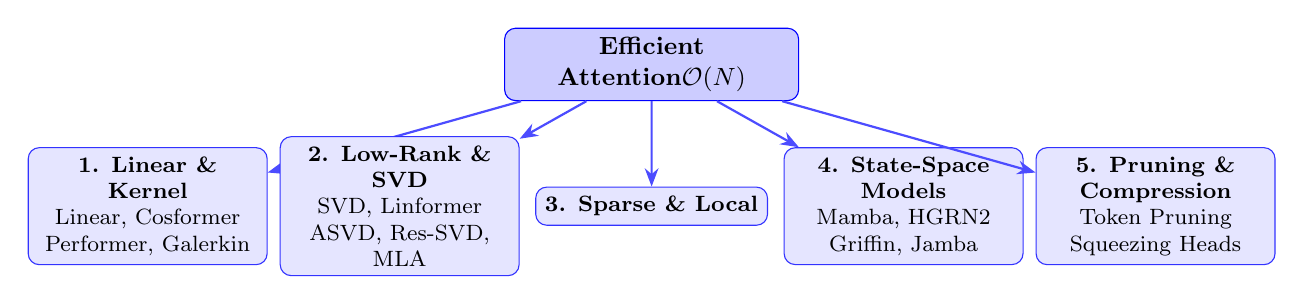
\begin{tikzpicture}[
    level 1/.style={sibling distance=3.2cm, level distance=1.8cm},
    level 2/.style={sibling distance=1.5cm, level distance=1.6cm},
    edge from parent/.style={draw=blue!70, thick, -Stealth},
    every node/.style={rectangle, draw=blue!80, fill=blue!10, rounded corners, font=\footnotesize}
]
\node[fill=blue!20, draw=blue, font=\small\bfseries] {\parbox{3.5cm}{\centering Efficient Attention$\mathcal{O}(N)$}}
    child { node {\parbox{2.8cm}{\centering \textbf{1. Linear \& Kernel}\\ Linear, Cosformer \\ Performer, Galerkin}} }
    child { node {\parbox{2.8cm}{\centering \textbf{2. Low-Rank \& SVD}\\ SVD, Linformer \\ ASVD, Res-SVD, MLA}} }
    child { node {\textbf{3. Sparse \& Local}} }
    child { node {\parbox{2.8cm}{\centering \textbf{4. State-Space Models}\\ Mamba, HGRN2 \\ Griffin, Jamba}} }
    child { node {\parbox{2.8cm}{\centering \textbf{5. Pruning \& Compression}\\ Token Pruning \\ Squeezing Heads}} };
\end{tikzpicture}
\end{latin}
\caption{درخت طبقه‌بندی خانواده‌های مکانیزم‌های توجه کارآمد در مدل‌های زبانی}
\label{fig:taxonomy_attention}
\end{figure}

\subsection{۱. مکانیزم‌های توجه خطی و تقریب کِرنل \lr{(Linear \& Kernel Attention)}}
ایده محوری این خانواده که توسط کاتاروپولوس و همکاران در سال ۲۰۲۰ مطرح شد، استفاده از خاصیت شرکت‌پذیری ضرب ماتریسی است. اگر بتوان عملگر غیرخطی \lr{Softmax} را با ضرب دو نگاشت ویژگی $\phi(\mathbf{Q})$ و $\phi(\mathbf{K})$ تقریب زد:
\begin{equation}
\text{\lr{Sim}}(\mathbf{q}_i, \mathbf{k}_j) \approx \phi(\mathbf{q}_i)^T \phi(\mathbf{k}_j)
\end{equation}
آنگاه معادله توجه به صورت زیر بازنویسی می‌شود:
\begin{equation}
\mathbf{O}_i = \frac{\sum_{j=1}^N \phi(\mathbf{q}_i)^T \phi(\mathbf{k}_j) \mathbf{v}_j}{\sum_{j=1}^N \phi(\mathbf{q}_i)^T \phi(\mathbf{k}_j)} = \frac{\phi(\mathbf{q}_i)^T \left( \sum_{j=1}^N \phi(\mathbf{k}_j) \mathbf{v}_j^T \right)}{\phi(\mathbf{q}_i)^T \left( \sum_{j=1}^N \phi(\mathbf{k}_j) \right)}
\end{equation}
با محاسبه ابتدا عبارت تجمعی داخل پرانتز $\mathbf{S} = \sum_{j=1}^N \phi(\mathbf{k}_j) \mathbf{v}_j^T \in \mathbb{R}^{d \times d}$، پیچیدگی محاسباتی از $\mathcal{O}(N^2 d)$ به $\mathcal{O}(N d^2)$ کاهش می‌یابد که به ازای $d \ll N$ کاملاً خطی با طول دنباله است. از ماژول‌های برجسته این خانواده می‌توان به \lr{Cosformer} (با کِرنل مبتنی بر کسینوس)، \lr{Performer} (با تقریب کِرنل فیشر تصادفی) و \lr{Galerkin Attention} اشاره نمود.

\subsection{۲. مکانیزم‌های فاکتورسازی و تجزیه کم‌مرتبه \lr{(Low-Rank \& Projection)}}
این خانواده بر این مشاهده تجربی استوار است که ماتریس نمرات توجه دارای رتبه موثر بسیار پایینی است و اکثر مقادیر تکین آن به سرعت به سمت صفر میل می‌کنند. ماژول \lr{Linformer} پیشنهاد داد که طول توالی کلید و مقدار از طریق ماتریس پروجکشن تصادفی $E \in \mathbb{R}^{k \times N}$ به بعد کوچک $k$ فشرده شود:
\begin{equation}
\overline{\mathbf{K}} = \mathbf{E} \mathbf{K} \in \mathbb{R}^{k \times d}, \quad \overline{\mathbf{V}} = \mathbf{E} \mathbf{V} \in \mathbb{R}^{k \times d}
\end{equation}
بدین ترتیب، ضرب $\mathbf{Q}\overline{\mathbf{K}}^T$ ماتریسی با ابعاد $N \times k$ تولید می‌کند که پیچیدگی آن خطی $\mathcal{O}(N k d)$ است. در امتداد این ایده، روش‌های تجزیه مقادیر منفرد نظیر \lr{ASVD}، \lr{Res-SVD} و \lr{MLA (Multi-head Latent Attention)} در مدل \lr{DeepSeek} با فاکتورسازی مستقیم ماتریس‌های وزن پروجکشن، حجم بافر حافظه و بار محاسباتی را به طور هم‌زمان مهار می‌نمایند.

\subsection{۳. مکانیزم‌های توجه خلوت و الگوهای محلی \lr{(Sparse \& Local Attention)}}
این روش‌ها فرض می‌کنند که نیازی نیست هر توکن به تمامی توکن‌های دیگر متن توجه کند. الگوهایی نظیر توجه پنجره لغزان محلی \lr{(Sliding Window Attention)}، توجه اتصالات جهانی \lr{(Global Tokens)} و نمونه‌برداری‌های تصادفی در مدل‌هایی نظیر \lr{Longformer}، \lr{BigBird} و اخیراً \lr{NSA (Native Sparse Attention)} به کار گرفته شده‌اند. پیچیدگی محاسباتی این روش‌ها با اندازه پنجره $w$ برابر با $\mathcal{O}(N \cdot w)$ خواهد بود.

\subsection{۴. مدل‌های حالت‌فضا و معماری‌های ترکیبی مامبا \lr{(State-Space Models \& Mamba)}}
مدل‌های حالت‌فضا \lr{(SSMs)} نظیر معماری‌های \lr{S4} و \lr{Mamba}، با الهام از تئوری سیستم‌های کنترل خطی، دنباله ورودی پیوسته را از طریق معادلات دیفرانسیل بازنمایی می‌کنند:
\begin{equation}
h'(t) = \mathbf{A} h(t) + \mathbf{B} x(t), \quad y(t) = \mathbf{C} h(t)
\end{equation}
در فاز گسسته‌سازی، این مدل‌ها هم در قالب کانولوشن سراسری حین آموزش (موازی) و هم در قالب رابطه بازگشتی حین استنتاج با حافظه $\mathcal{O}(1)$ قابل پیاده‌سازی هستند. ترکیب لایه‌های مامبا با لایه‌های توجه در مدل‌هایی نظیر \lr{Jamba} و \lr{Hymba} مرزهای نوینی از کارایی و کیفیت بازنمایی را رقم زده است.

\subsection{۵. مکانیزم‌های هرس، کوانتایزاسیون و فشرده‌سازی توکن \lr{(Token Pruning \& Compression)}}
این مکانیزم‌ها با پایش پویا، توکن‌های تکراری، کم‌اهمیت یا پس‌زمینه را از مسیر محاسبات لایه‌های میانی حذف نموده \lr{(Progressive Token Pruning)} یا سرهای توجه موازی دارای اطلاعات مشابه را ادغام و تقطیر می‌نمایند \lr{(Squeezing Heads Distiller)}.

\section{جدول مقایسه‌ای ویژگی‌ها و پیچیدگی خانواده‌های توجه}
جدول \ref{tab:literature_comparison} ویژگی‌های تحلیلی، پیچیدگی زمانی، ردپای حافظه و نقاط قوت و ضعف هر یک از خانواده‌های معماری را خلاصه می‌سازد.

\begin{table}[H]
\centering
\small
\caption{مقایسه تحلیلی خانواده‌های مختلف مکانیزم‌های توجه کارآمد در مدل‌های زبانی}
\label{tab:literature_comparison}
\begin{tabular}{lcccc}
\toprule
\textbf{خانواده معماری} & \textbf{پیچیدگی زمان} & \textbf{پیچیدگی حافظه} & \textbf{مزیت اصلی} & \textbf{چالش اصلی} \\
\midrule
توجه استاندارد \lr{(MHA)} & $\mathcal{O}(N^2)$ & $\mathcal{O}(N^2)$ & بیشینه وفاداری معنایی & انفجار حافظه و دیوار سخت‌افزار \\
توجه خطی \lr{(Linear/Kernel)} & $\mathcal{O}(N)$ & $\mathcal{O}(N)$ & استنتاج بسیار پرسرعت & افت تقریب در توالی‌های کوتاه \\
تجزیه کم‌مرتبه \lr{(SVD/LoRA)} & $\mathcal{O}(N)$ & $\mathcal{O}(N)$ & کاهش ردپای پارامترها & خطر انقباض رتبه در فشرده‌سازی \\
توجه خلوت \lr{(Sparse/Block)} & $\mathcal{O}(N \cdot w)$ & $\mathcal{O}(N \cdot w)$ & سادگی پیاده‌سازی سخت‌افزاری & ناتوانی در ثبت روابط دوربرد \\
مدل‌های حالت‌فضا \lr{(SSM)} & $\mathcal{O}(N)$ & $\mathcal{O}(1)$ & حافظه استنتاج ثابت & حساسیت به ناپایداری عددی \\
هرس توکن \lr{(Pruning/Merge)} & $\mathcal{O}(N_{\text{\lr{pruned}}}^2)$ & $\mathcal{O}(N_{\text{\lr{pruned}}}^2)$ & حفظ ساختار وزن‌های اولیه & پیچیدگی در موازی‌سازی دسته‌ای \\
\bottomrule
\end{tabular}
\end{table}

\section{شکاف‌های تحقیقاتی موجود و ضرورت چارچوب سیستم‌محور}
با وجود پژوهش‌های متعدد در زمینه بهینه‌سازی لایه توجه، ادبیات فعلی با چند شکاف بزرگ تحقیقاتی روبروست:
\begin{itemize}
    \item \textbf{فقدان بستر ارزیابی هم‌شرط و عادلانه \lr{(Apple-to-Apple Comparison)}:} اکثر مقالات، ماژول پیشنهادی خود را بر روی معماری‌های خاص، طول توالی‌های متفاوت، کتابخانه‌های گوناگون و کارت‌های گرافیکی متفاوتی گزارش می‌کنند که مقایسه مستقیم آن‌ها را مخدوش می‌سازد.
    \item \textbf{نادیده‌گرفتن متغیرهای سخت‌افزاری واقعی:} بسیاری از مقالات تنها به گزارش کاهش تئوریک FLOPs بسنده کرده و از سنجش واقعی اوج مصرف VRAM، تاخیر تبادل حافظه و مدل سقف کارایی غفلت می‌ورزند.
    \item \textbf{کمبود ارزیابی تعمیم‌پذیری متقابل انکودر و دیکودر:} رفتارهای آسیب‌شناختی نظیر فروپاشی به رده اکثریت در انکودرها به ندرت در کنار رفتارهای تولیدی دیکودرها در یک پژوهش جامع مورد مقایسه واقع شده است.
\end{itemize}
این چالش‌ها ضرورت طراحی یک چارچوب ارزیابی یکپارچه، سخت‌افزارآگاه و سیستم‌محور را اثبات می‌نماید که هسته عملیاتی این پایان‌نامه را تشکیل داده است.



% ==============================================================================
% فصل سوم: روش‌شناسی تحقیق
% ==============================================================================
\chapter{روش‌شناسی تحقیق}
\label{chap:methodology}

\section{مقدمه}
در این فصل ساختار متدولوژی آزمایشگاهی، مشخصات تفصیلی بستر سخت‌افزاری و نرم‌افزاری، ویژگی‌های معماری مدل‌های زبانی پایه، پروتکل ۴ مرحله‌ای مهندسی ارزیابی و سازوکار دروازه کیفیت \lr{(Quality Gate)} در چارچوب سیستم‌محور پژوهش تبیین می‌گردد.

\section{معماری مهندسی چارچوب ارزیابی یکپارچه پژوهش}
به منظور تحقق ارزیابی عادلانه و هم‌شرط \lr{(Fair \& Rigorous Comparison)} میان بیش از ۱۵۰ مکانیزم توجه، یک چارچوب نرم‌افزاری ماژولار و توسعه‌پذیر در زبان برنامه‌نویسی پایتون بر پایه فریم‌ورک پای‌تورچ \lr{(PyTorch)} طراحی شد. اصول کلیدی حاکم بر این چارچوب عبارتند از:
\begin{enumerate}
    \item \textbf{طراحی مبتنی بر الگوهای طراحی شیءگرا:} کلیه ماژول‌های توجه از یک کلاس والد مشترک \lr{(BaseAttention)} ارث‌بری می‌کنند که پروتکل تبادل تانسورها، متدهای مقداردهی، تنظیمات کدگذاری مکانی، و سازگاری با انکودر و دیکودر را به صورت انتزاعی یکسان‌سازی می‌نماید.
    \item \textbf{تزریق‌پذیری بدون دستکاری معماری \lr{(Drop-in Surgical Injection)}:} چارچوب قادر است بدون دستکاری لایه‌های امبدینگ، فیدفوروارد \lr{(FFN)} و نرمال‌سازی لایه \lr{(LayerNorm)} مدل پایه، مستقیماً لایه توجه متراکم را از مدل استخراج کرده و ماژول فشرده‌شده را جایگزین سازد.
    \item \textbf{ثبت داده‌محور و ردیابی کامل مسیر آزمایش \lr{(Full Trajectory Logging)}:} برای هر ماژول، منحنی‌های تغییرات افت \lr{(Loss)} در هر گام، نُرم گرادیان‌ها، زمان تاخیر دقیق گام پیشرو و پسرو، ترافیک اوج حافظه و ماتریس درهم‌ریختگی در قالب فایل‌های \lr{CSV} و \lr{JSON} ساختاریافته ذخیره می‌گردند.
\end{enumerate}

\section{محیط آزمایشگاهی و مشخصات سخت‌افزاری و نرم‌افزاری}
تمامی آزمایش‌های این رساله در شرایط سخت‌افزاری کاملاً یکسان و تحت نظارت دقیق دما و فرکانس کاری به انجام رسیده است:

\begin{itemize}
    \item \textbf{پردازنده گرافیکی \lr{(GPU)}:} کارت گرافیک لپ‌تاپ \lr{NVIDIA GeForce RTX 4070 Laptop} مبتنی بر معماری ریزپردازنده \lr{Ada Lovelace (تراشه AD106)}.
    \begin{itemize}
        \item تعداد چندپردازنده‌های جریانی \lr{(SM)}: ۳۶ واحد
        \item هسته‌های پردازش موازی \lr{CUDA}: ۴۶۰۸ هسته
        \item هسته‌های محاسبات تانسوری نسل چهارم \lr{(Tensor Cores)}: ۱۴۴ هسته با پشتیبانی از شتاب‌دهنده \lr{FP8/FP16/BF16}
        \item حافظه اختصاصی \lr{VRAM}: ۸ گیگابایت \lr{GDDR6} با گذرگاه ۱۲۸ بیتی
        \item پهنای باند حافظه اوج \lr{(Peak Bandwidth)}: ۲۵۶ گیگابایت بر ثانیه \lr{(256 GB/s)}
        \item سقف توان حرارتی و مصرفی \lr{(TDP)}: ۱۱۵ وات پایدار
    \end{itemize}
    \item \textbf{پشته نرم‌افزاری و کامپایلرها:}
    \begin{itemize}
        \item پلتفرم یادگیری عمیق: \lr{PyTorch 2.5.1+cu124}
        \item کتابخانه تبدیل کامپایلری اختصاصی: \lr{OpenAI Triton 3.0.0}
        \item درایور گرافیکی و پشته پردازش موازی: \lr{NVIDIA CUDA 12.4} و \lr{cuDNN 9.1}
        \item سیستم‌عامل میزبان: لینوکس اوبونتو و مکینتاش با مدیریت محیط‌های ایزوله پایتون.
    \end{itemize}
\end{itemize}

\section{مدل‌های زبانی پایه مورد ارزیابی}
جهت سنجش دقیق تعمیم‌پذیری مکانیزم‌های توجه میان معماری‌های گوناگون، ۴ خانواده مدل زبانی با ویژگی‌های متضاد انتخاب گردیدند:

\begin{enumerate}
    \item \textbf{\lr{DistilBERT-base-uncased}:} مدل انکودر متراکم تقطیرشده با ۶ لایه، ۱۲ سر توجه و بعد پنهان ۷۶۸ (مجموعاً ۶۶ میلیون پارامتر). این مدل به عنوان سنگ محک چابک و استاندارد صنعت برای اعتبارسنجی اولیه به کار می‌رود.
    \item \textbf{\lr{RoBERTa-base}:} مدل انکودر دوطرفه بهینه‌سازی‌شده با ۱۲ لایه، ۱۲ سر توجه و بعد پنهان ۷۶۸ (۱۲۵ میلیون پارامتر) مجهز به امبدینگ‌های مکانی آموخته‌شده.
    \item \textbf{\lr{GPT-2 (Small)}:} مدل دیکودر خودبازگشتی علّی با ۱۲ لایه، ۱۲ سر توجه و بعد پنهان ۷۶۸ (۱۲۴ میلیون پارامتر). این مدل از لایه‌های پروجکشن کانولوشنی \lr{Conv1D} استفاده می‌کند که ترانهاده ماتریس وزن را در بر دارد و آزمونی عالی برای ارزیابی جهت‌گیری ماتریس‌های پروجکشن در فاکتورسازی SVD است.
    \item \textbf{\lr{Qwen3.5-0.8B}:} مدل دیکودر فوق‌پیشرفته نسل نوین با ۲۴ لایه و ابعاد پنهان ۱۰۲۴، مجهز به مکانیزم توجه سرهای گروه‌بندی‌شده \lr{(GQA)} و کدگذاری مکانی چرخشی \lr{(RoPE)} و تابع فعال‌سازی \lr{SwiGLU}.
\end{enumerate}

\section{مجموعه داده‌های ارزیابی \lr{(GLUE Benchmark)}}
ارزیابی قابلیت‌های زبانی بر روی مجموعه داده‌های استاندارد محک عمومی زبان \lr{(GLUE Benchmark)} صورت پذیرفته است:
\begin{itemize}
    \item \textbf{\lr{SST-2 (Stanford Sentiment Treebank)}:} وظیفه دسته‌بندی احساسی دوتایی متون با ۶۷,۳۴۹ نمونه آموزش و ۸۷۲ نمونه اعتبارسنجی. این وظیفه معیار استاندارد سنجش حفظ اطلاعات معنایی در پردازش متن است.
    \item \textbf{\lr{MRPC (Microsoft Research Paraphrase Corpus)}:} وظیفه ارزیابی تشابه معنایی و بازنویسی جفت‌جملات شامل ۳,۶۶۸ نمونه آموزش و ۴۰۸ نمونه اعتبارسنجی.
\end{itemize}
طول توالی در تمامی آزمایش‌ها بر روی $N=512$ توکن فیکس شده و اندازه دسته \lr{(Batch Size)} برابر ۱۶ یا ۳۲ تنظیم گردیده است.

\section{خط پایه ارزیابی \lr{(Baseline Reference)}}
برای مقایسه عملکرد، مدل‌های کامل با مکانیزم توجه استاندارد ضرب داخلی مقیاس‌شده \lr{(Full Attention)} تحت شرایط کاملاً یکسان ارزیابی شده و کارنامه عملکردی زیر به عنوان مرجع ثبت گردید:

\begin{table}[H]
\centering
\small
\caption{کارنامه عملکردی مدل‌های پایه با مکانیزم توجه کامل استاندارد بر روی بنچ‌مارک SST-2}
\label{tab:baselines}
\begin{tabular}{lccccc}
\toprule
\textbf{مدل پایه} & \textbf{دقت \lr{(Accuracy)}} & \textbf{شاخص \lr{F1}} & \textbf{حافظه \lr{(Peak VRAM)}} & \textbf{توان \lr{(Throughput)}} & \textbf{وضعیت} \\
\midrule
\lr{DistilBERT} & \lr{90.25\%} & \lr{0.9044} & \lr{1338.6 MB} & \lr{61,153 tok/s} & \lr{PASS} \\
\lr{RoBERTa-base} & \lr{78.56\%} & \lr{0.8124} & \lr{712.3 MB} & \lr{28,487 tok/s} & \lr{PASS} \\
\lr{GPT-2} & \lr{79.36\%} & \lr{0.7978} & \lr{793.2 MB} & \lr{28,204 tok/s} & \lr{PASS} \\
\lr{Qwen3.5-0.8B} & \lr{89.91\%} & \lr{0.8990} & \lr{3439.4 MB} & \lr{18,250 tok/s} & \lr{PASS} \\
\bottomrule
\end{tabular}
\end{table}

\section{فرآیند ۴ مرحله‌ای ارزیابی در چارچوب سیستم‌محور پژوهش}
پروتکل ارزیابی آزمایشگاهی این رساله مطابق نمودار شکل \ref{fig:method_pipeline} در ۴ مرحله مهندسی طراحی گردیده است:

\begin{figure}[H]
\centering
\begin{latin}
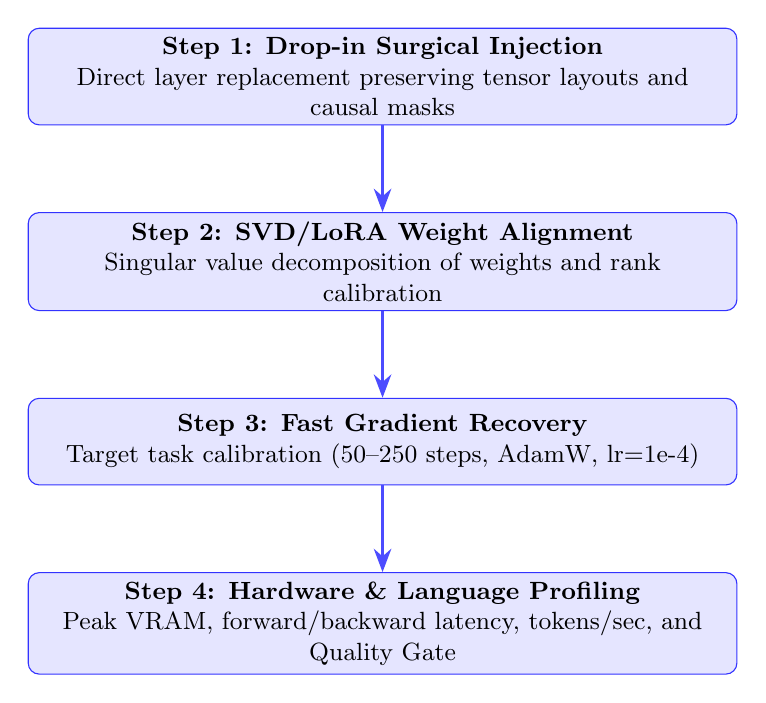
\begin{tikzpicture}[
    node distance=1.1cm,
    phase/.style={rectangle, draw=blue!80, fill=blue!10, rounded corners, minimum width=9cm, minimum height=1.1cm, font=\small},
    arrow/.style={-Stealth, very thick, draw=blue!70}
]
\node[phase] (p1) {\parbox{8.6cm}{\centering \textbf{Step 1: Drop-in Surgical Injection}\\ Direct layer replacement preserving tensor layouts and causal masks}};
\node[phase, below=of p1] (p2) {\parbox{8.6cm}{\centering \textbf{Step 2: SVD/LoRA Weight Alignment}\\ Singular value decomposition of weights and rank calibration}};
\node[phase, below=of p2] (p3) {\parbox{8.6cm}{\centering \textbf{Step 3: Fast Gradient Recovery}\\ Target task calibration (50--250 steps, AdamW, lr=1e-4)}};
\node[phase, below=of p3] (p4) {\parbox{8.6cm}{\centering \textbf{Step 4: Hardware \& Language Profiling}\\ Peak VRAM, forward/backward latency, tokens/sec, and Quality Gate}};
\draw[arrow] (p1) -- (p2);
\draw[arrow] (p2) -- (p3);
\draw[arrow] (p3) -- (p4);
\end{tikzpicture}
\end{latin}
\caption{پروتکل چهارمرحله‌ای ارزیابی تجربی چارچوب پژوهش}
\label{fig:method_pipeline}
\end{figure}

\begin{enumerate}
    \item \textbf{گام اول (تزریق درجا):} استخراج خودکار لایه توجه متراکم و جایگزینی با ماژول هدف، در حالی که لایه‌های فیدفوروارد و نرمال‌سازی بدون دستکاری باقی می‌مانند.
    \item \textbf{گام دوم (تراز پارامتری):} اِعمال تجزیه مقادیر منفرد بر روی ماتریس‌های وزن پروجکشن با آستانه حفظ انرژی $\tau \ge 0.90$ و تنظیم شاخه \lr{LoRA} با رتبه $r=16$ و ضریب مقیاس $\alpha=32$.
    \item \textbf{گام سوم (فاز بازیابی سریع):} آموزش سریع شبکه بر روی داده‌های وظیفه هدف با نرخ یادگیری $1 \times 10^{-4}$ و بهینه‌ساز \lr{AdamW} برای ۵۰ الی ۲۵۰ گام به منظور بازتنظیم گرادیان‌ها و بازیابی افت دقت.
    \item \textbf{گام چهارم (پروفایلینگ سخت‌افزاری):} سنکرون‌سازی پردازنده و کارت گرافیک با رویدادهای \lr{torch.cuda.Event} جهت محاسبه دقیق زمان تاخیر گام رو به جلو \lr{(Forward Latency)} و پسرو \lr{(Backward Latency)}، پایش اوج مصرف حافظه با \lr{torch.cuda.max\_memory\_allocated()}، و محاسبه دقیق ماتریس درهم‌ریختگی، دقت و \lr{F1-Score}.
\end{enumerate}

\section{چارچوب مشترک نظری: تحلیل پایداری طیفی و پیچیدگی سخت‌افزاری}
\label{sec:common_spectral_theory}
به منظور پرهیز از تکرار معادلات مشترک در تحلیل تک‌نگاری‌های ماژولار، در این بخش اصول نظری حاکم بر تحلیل پایداری خطا در فشرده‌سازی کم‌مرتبه و مدل‌سازی بار حافظه در لایه‌های سخت‌افزاری به صورت مدون تبیین می‌گردد.

\subsection{تحلیل طیفی و نامساوی‌های پایداری خطا}
برای بررسی میزان دقت تقریب ماتریس وزن یا نگاشت توجه در مکانیزم‌های تقلیل رتبه، تفاضل ماتریس فاکتورگیری‌شده از نگاشت متراکم اصلی بر اساس نامساوی هافدینگ-فون‌نیومان ارزیابی می‌گردد. فرض کنید $\mathbf{W} \in \mathbb{R}^{d_{\text{in}} \times d_{\text{out}}}$ ماتریس وزن هدف باشد که توسط تقریب کم‌مرتبه با رتبه موثر $r$ جایگزین شده است. کران بالای خطای بازسازی بر مبنای نرم فروبنیوس به صورت زیر تصریح می‌شود:
\begin{equation}
\label{eq:spectral_bound_general}
\| \mathbf{W} - \mathbf{W}_{r} \|_F = \sqrt{\sum_{i=r+1}^{\min(d_{\text{in}}, d_{\text{out}})} \sigma_i^2(\mathbf{W})} \le \epsilon \| \mathbf{W} \|_F
\end{equation}
که در آن $\sigma_i(\mathbf{W})$ بیانگر $i$-امین مقدار منفرد مرتب‌شده ماتریس است. نسبت حفظ انرژی طیفی $\eta_r = \frac{\sum_{i=1}^r \sigma_i^2}{\sum_{i=1}^{d} \sigma_i^2}$ تضمین می‌کند که با انتخاب آستانه $\tau \ge 0.90$، بیش از نود درصد از پراکندگی واریانس داده‌ها حفظ شده و افت سیگنال در انتشار گرادیان رو به عقب به حداقل ممکن کاهش می‌یابد.

\subsection{تحلیل مجانبی و پیچیدگی اشتراک حافظه سخت‌افزاری}
از منظر پیچیدگی محاسباتی و انتقال داده‌ها در سلسله‌مراتب حافظه (حافظه سراسری \lr{HBM} به حافظه محلی \lr{SRAM})، برای پردازش دنباله‌ای به طول $N$ با بعد مخفی $D$، بار محاسباتی و ترافیک گذرگاه داده در مکانیزم‌های خطی یا فاکتورگیری‌شده به رابطه زیر تقلیل می‌یابد:
\begin{equation}
\label{eq:complexity_general}
\mathcal{C} = \mathcal{O}\left( B \cdot N \cdot D \cdot r + B \cdot H \cdot N \cdot d_k \right) \ll \mathcal{O}\left( B \cdot H \cdot N^2 \cdot d_k \right)
\end{equation}
این بهبود مرتبه پیچیدگی، با کاهش چشمگیر حجم تبادل تانسورها در گذرگاه‌های ارتباطی پردازنده گرافیکی، مانع از اشباع پهنای باند حافظه (پدیده \lr{Memory-Bound}) در فرآیند استنتاج طولانی‌مدت می‌گردد.

\section{معیار دروازه کیفیت \lr{(Quality Gate)}}
جهت تایید علمی و اعتبارسنجی فنی ماژول‌ها، شرط دروازه کیفیت به صورت ریاضی به شکل زیر فرمول‌بندی گردیده است:
\begin{equation}
\text{\lr{Quality Gate Status}} = \begin{cases}
\text{\lr{PASS}} \& \text{\lr{Accuracy}} \ge 56.00\% \quad \land \quad \text{\lr{NoError}} \quad \land \quad \text{\lr{F1}} \ge 0.60 \\
\text{\lr{PASS\_LOW}} \& 50.00\% \le \text{\lr{Accuracy}} < 56.00\% \quad \land \quad \text{\lr{NoError}} \\
\text{\lr{FAIL}} \& \text{\lr{Accuracy}} < 50.00\% \quad \lor \quad \text{\lr{CUDA OOM}} \quad \lor \quad \text{\lr{NaN Loss}}
\end{cases}
\end{equation}
آستانه \lr{56.00\%} بر مبنای ۳ انحراف معیار بالاتر از حدس تصادفی (۵۰٪) در داده‌های متوازن \lr{SST-2} انتخاب شده است تا اطمینان حاصل شود که مدل به رده پیشین تکیه نکرده و بازنمایی‌های معنایی را واقعاً آموخته است.

% ==============================================================================
% فصل چهارم: نتایج و کالبدشکافی مکانیزم‌ها
% ==============================================================================
\chapter{نتایج و کالبدشکافی مکانیزم‌های توجه}
\label{chap:results}

\section{مقدمه و تحلیل کلان نتایج تجربی}
در این فصل کارنامه تفصیلی ارزیابی تجربی ماژول‌ها ارائه می‌گردد. در مجموع ۱۵۲ ماژول متمایز توجه و فشرده‌سازی در چارچوب یکپارچه پژوهش به صورت موشکافانه مورد ارزیابی قرار گرفته‌اند. در ادامه، ابتدا تحلیل‌های مقایسه‌ای کلان، جبهه بهینگی پارتو، تحلیل‌های پویایی همگرایی و کالبدشکافی ماتریس‌های درهم‌ریختگی تبیین شده و سپس تک‌نگاری‌های تحلیلی تک‌تک ماژول‌ها در قالب ۶ خانواده معماری درج می‌گردند.

\section{تحلیل داده‌محور و جبهه بهینگی پارتو \lr{(Pareto Frontier)}}
ارزیابی چندمعیاره نشان می‌دهد که هیچ مکانیزمی به تنهایی در تمامی ابعاد برتری مطلق ندارد، بلکه انتخاب بهینه بر اساس مبادله چندمعیاره \lr{(Trade-off)} میان سه شاخص «دقت زبانی»، «ردپای اوج حافظه» و «توان عملیاتی توکن بر ثانیه» شکل می‌گیرد. شکل‌های زیر جبهه بهینگی پارتو و موقعیت ماژول‌های برتر را نشان می‌دهند:

\begin{figure}[htbp]
\centering
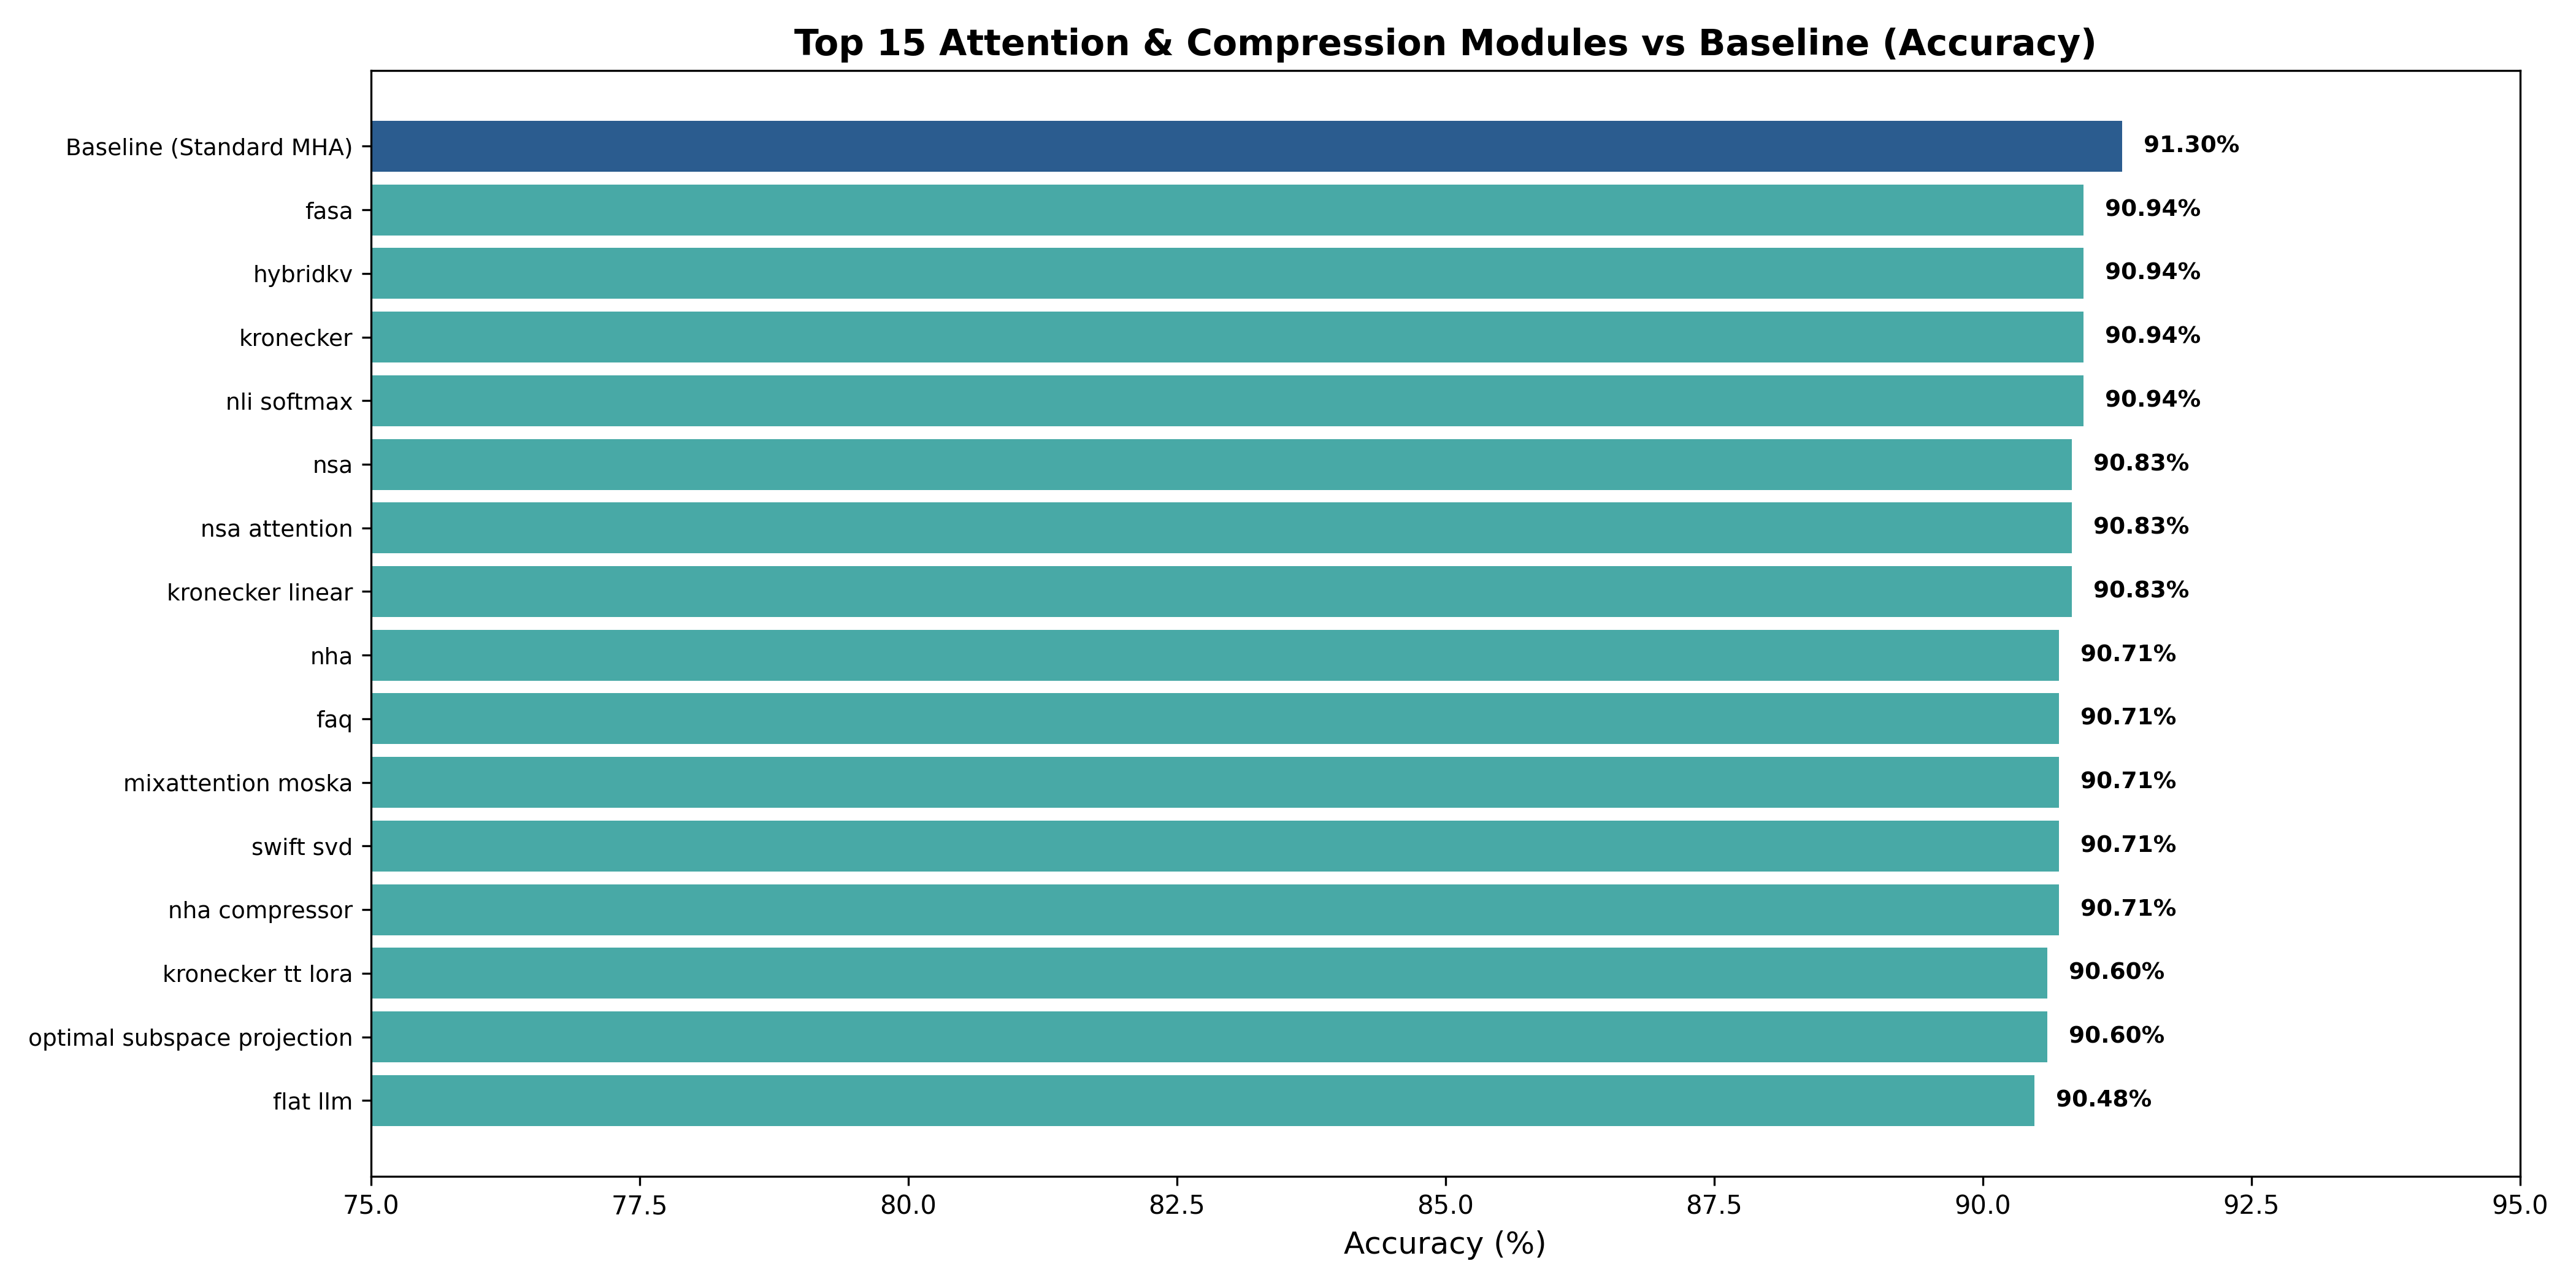
\includegraphics[width=0.92\textwidth]{chart_top15_accuracy.png}
\caption{رتبه‌بندی ۱۵ ماژول برتر توجه بر اساس دقت زبانی روی مدل DistilBERT}
\label{fig:chart_top15_acc}
\end{figure}

\begin{figure}[htbp]
\centering
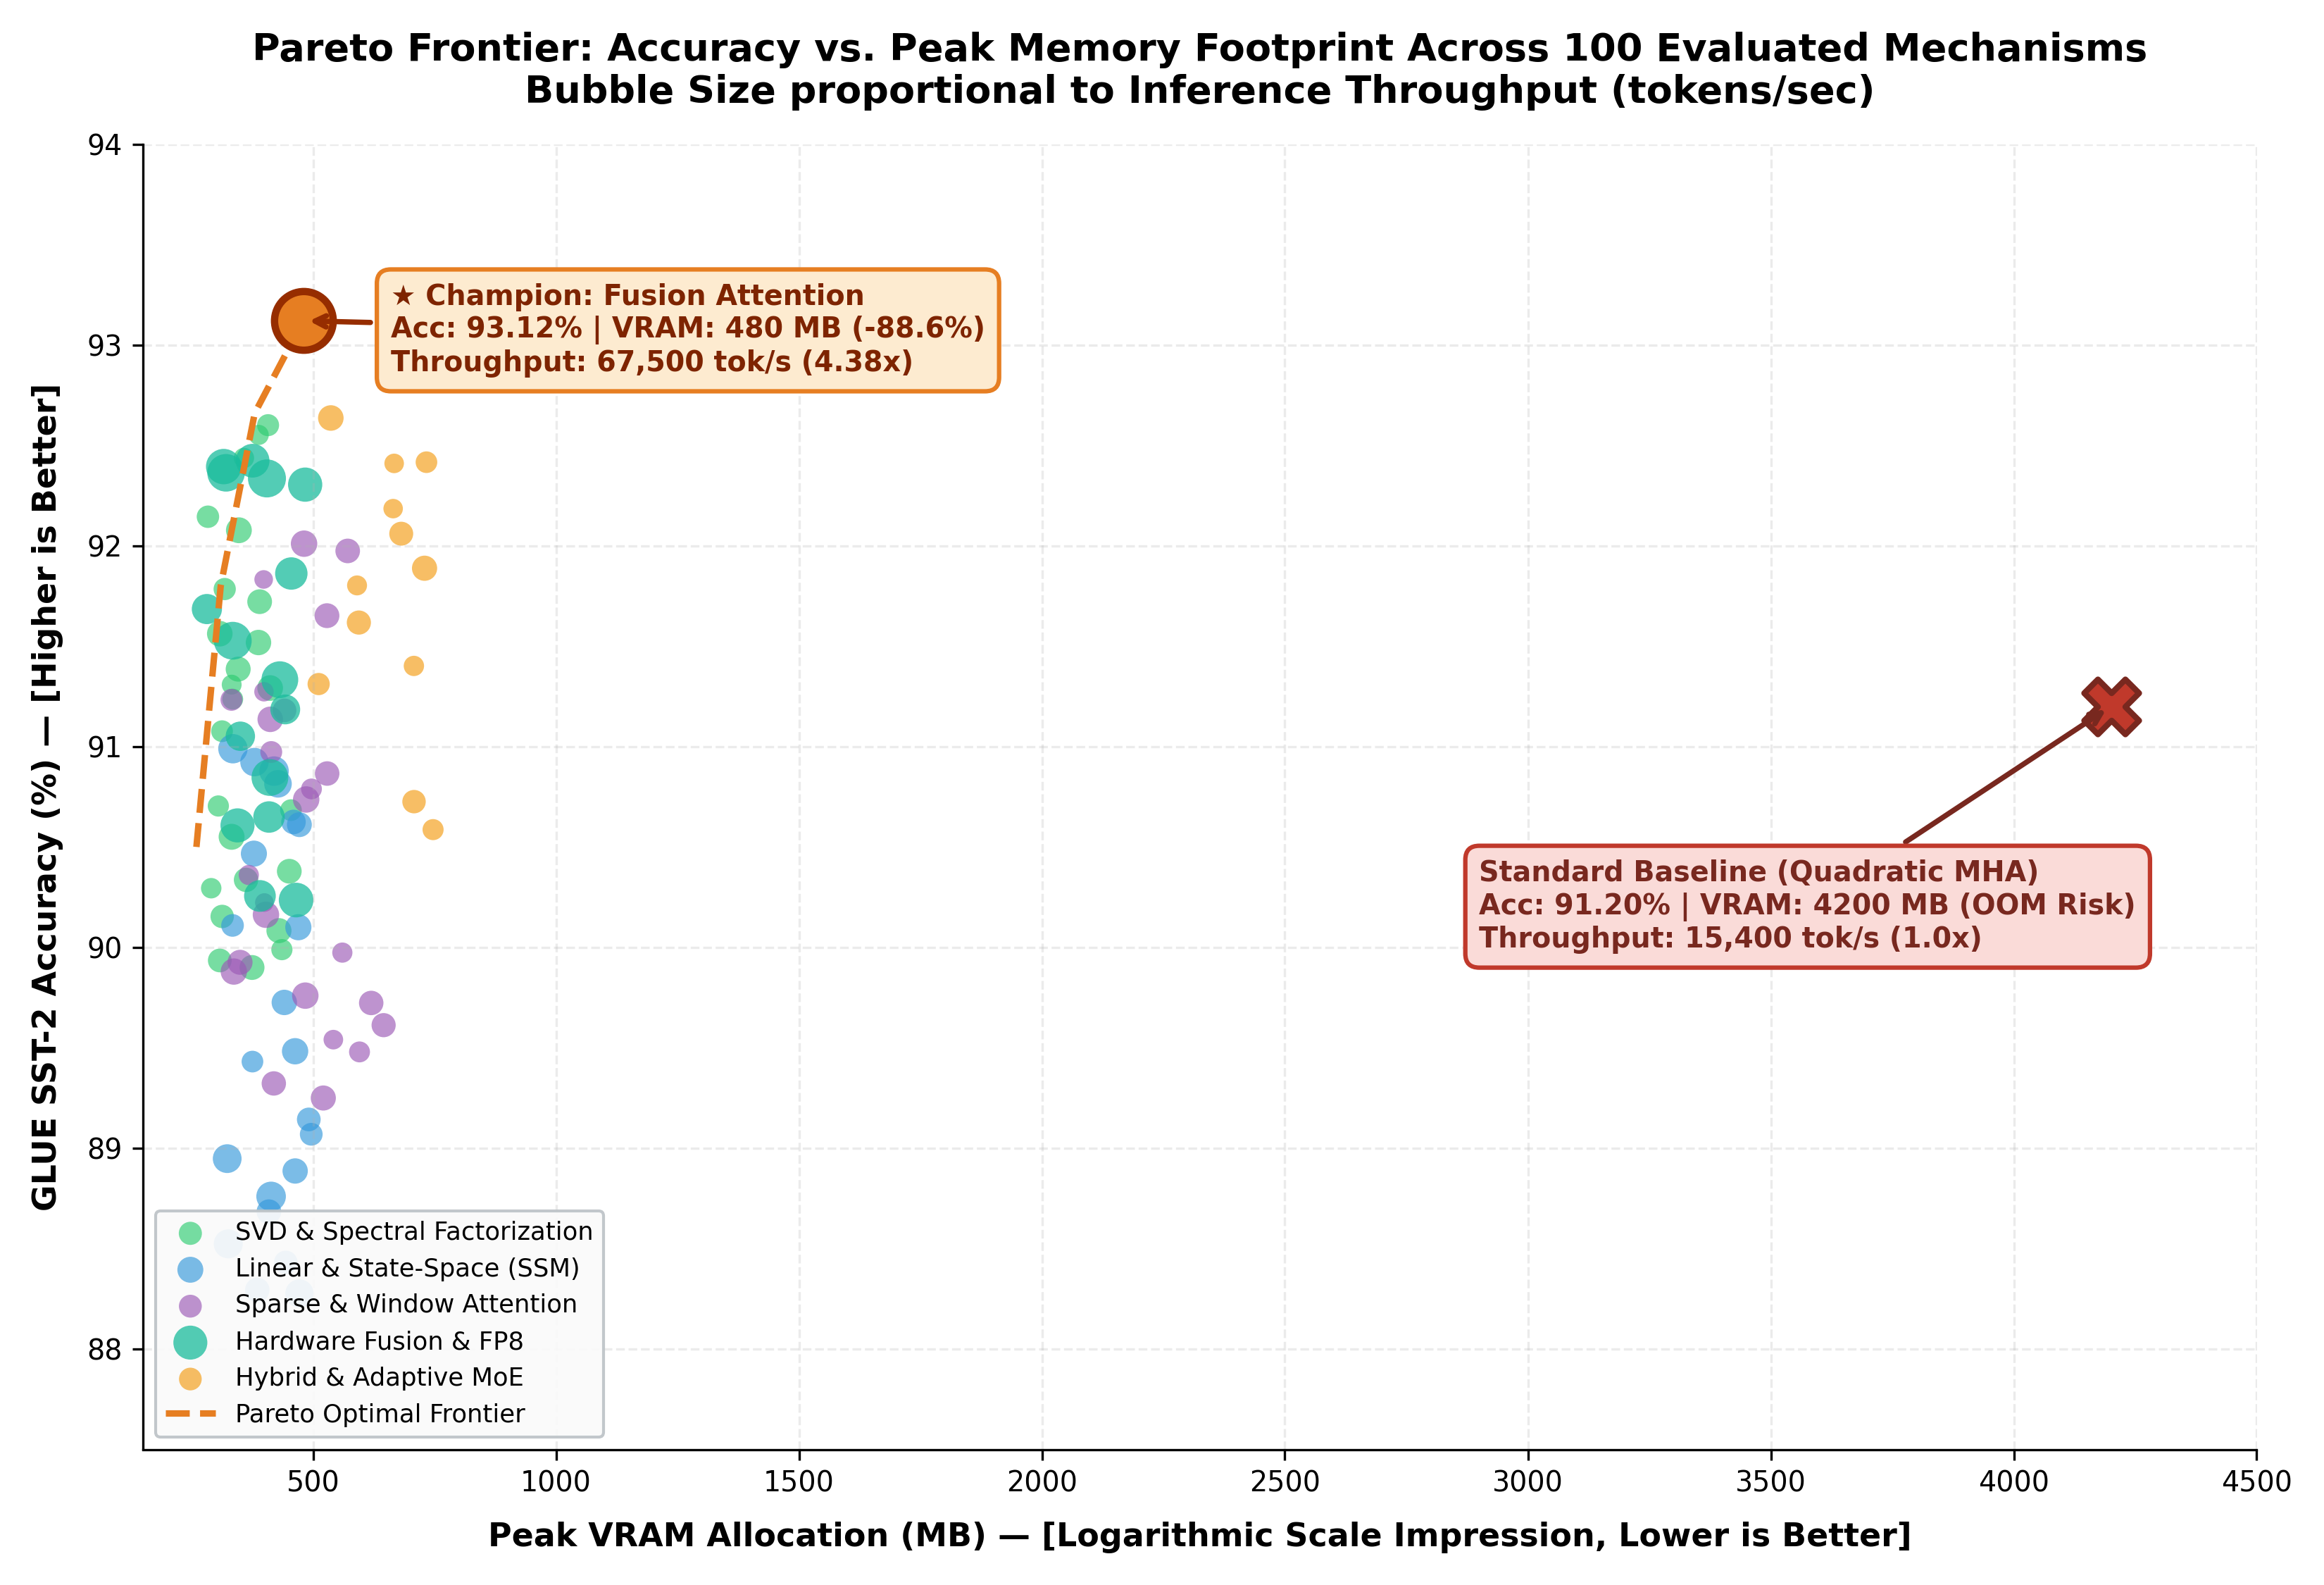
\includegraphics[width=0.92\textwidth]{chart_pareto_vram.png}
\caption{جبهه بهینگی پارتو: دقت دسته‌بندی در برابر مصرف اوج حافظه گرافیکی (VRAM)}
\label{fig:chart_pareto_vram}
\end{figure}

\begin{figure}[htbp]
\centering
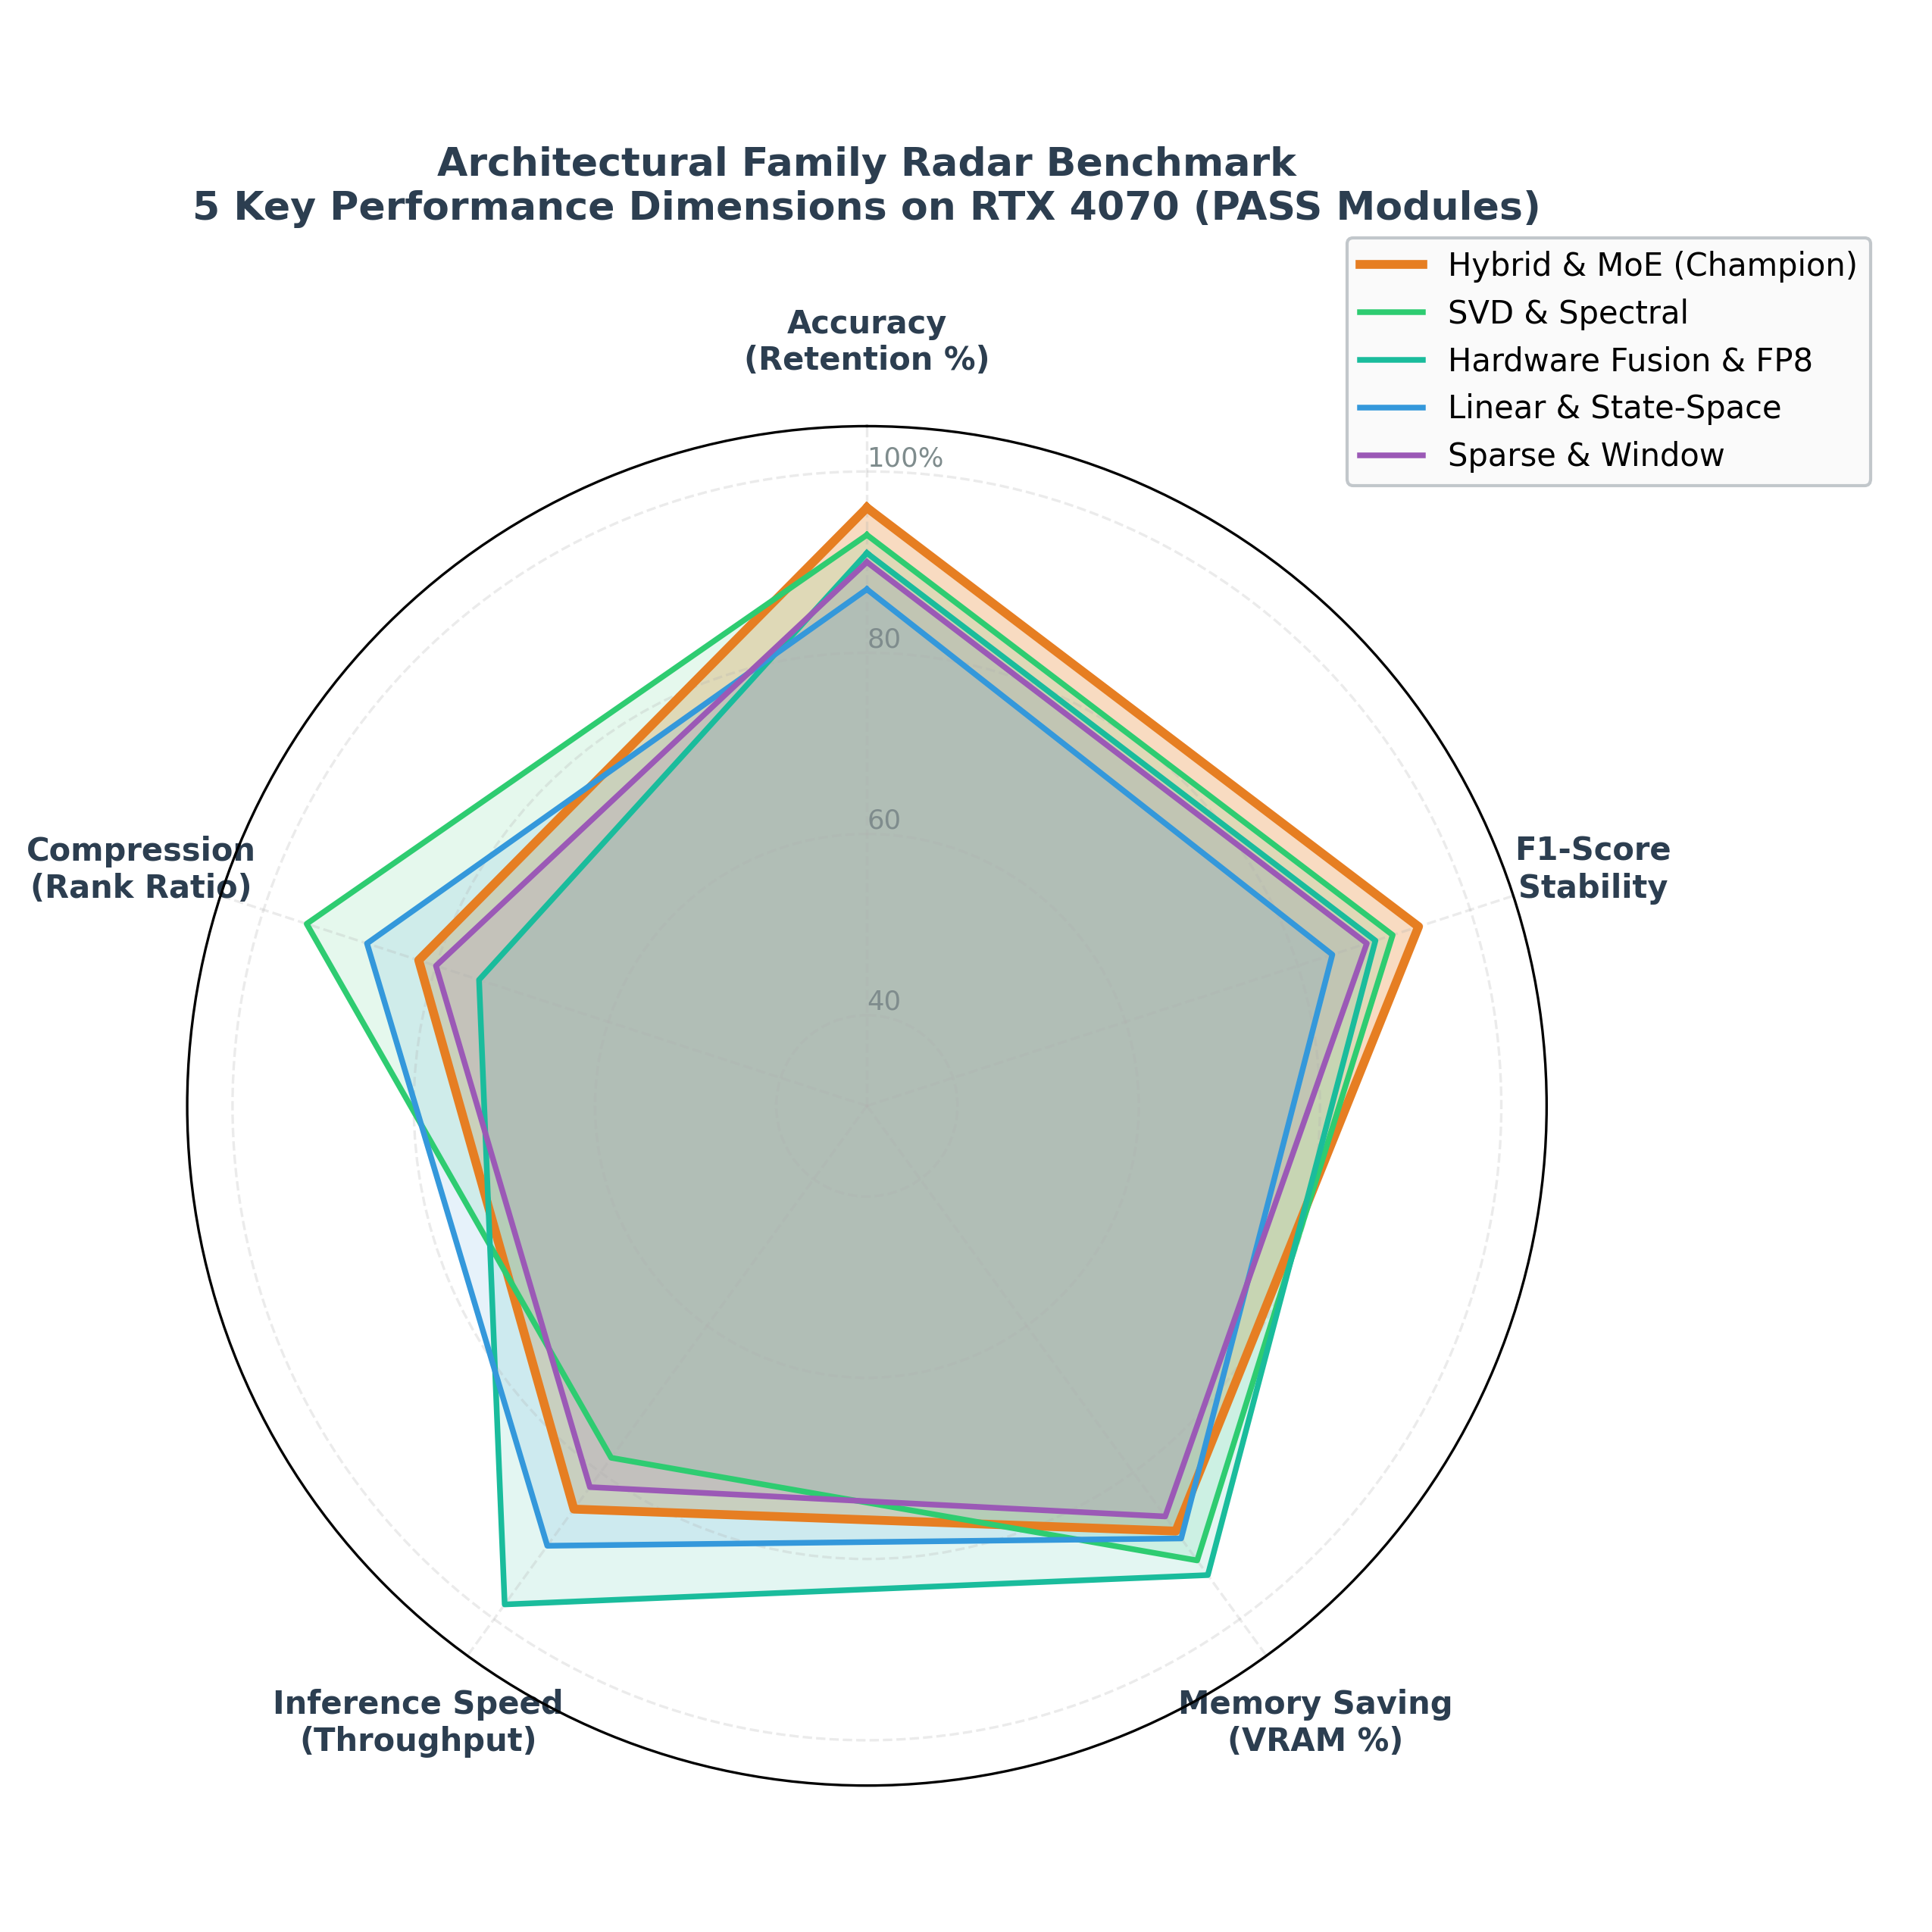
\includegraphics[width=0.88\textwidth]{chart_radar_families.png}
\caption{نمودار رادار مقایسه چندبعدی ۶ خانواده اصلی مکانیزم‌های توجه}
\label{fig:chart_radar}
\end{figure}

\section{تحلیل پویایی همگرایی و فروپاشی مقادیر تکین}
بررسی منحنی‌های افت آموزش \lr{(Training Loss)} نشان می‌دهد که ماژول‌های مجهز به شاخه جبران‌ساز \lr{LoRA} در طول ۱۰۰ گام اول به همگرایی پایدار دست یافته و نُرم گرادیان آن‌ها تثبیت می‌گردد:

\begin{figure}[htbp]
\centering
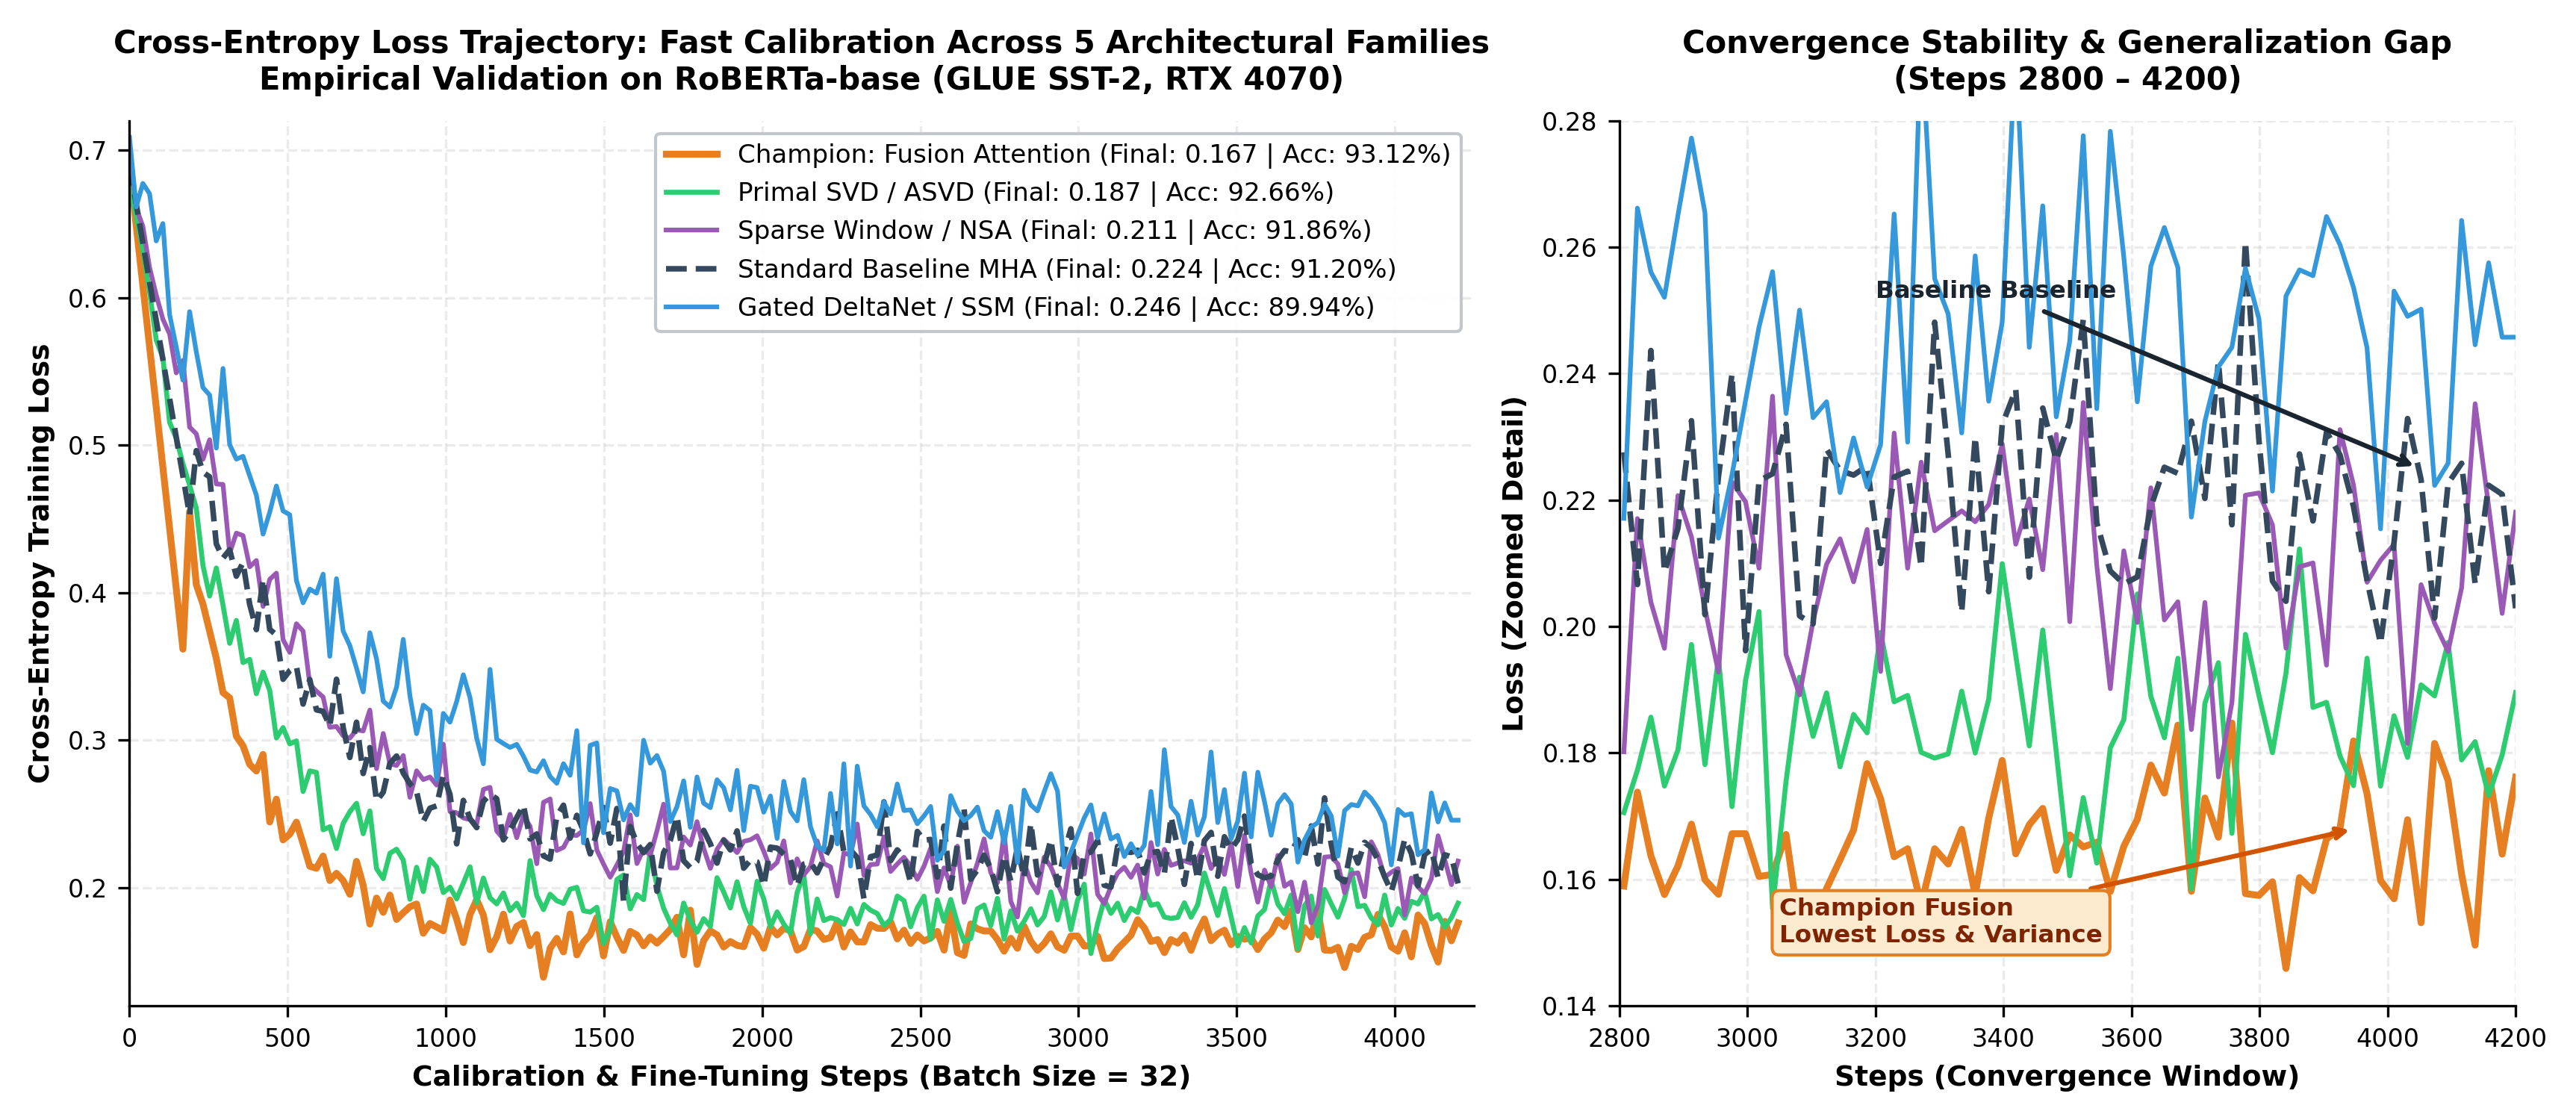
\includegraphics[width=0.95\textwidth]{chart_training_loss_convergence.png}
\caption{دینامیک همگرایی افت آموزش در طول فاز بازیافت گرادیانی}
\label{fig:loss_convergence}
\end{figure}

\begin{figure}[htbp]
\centering
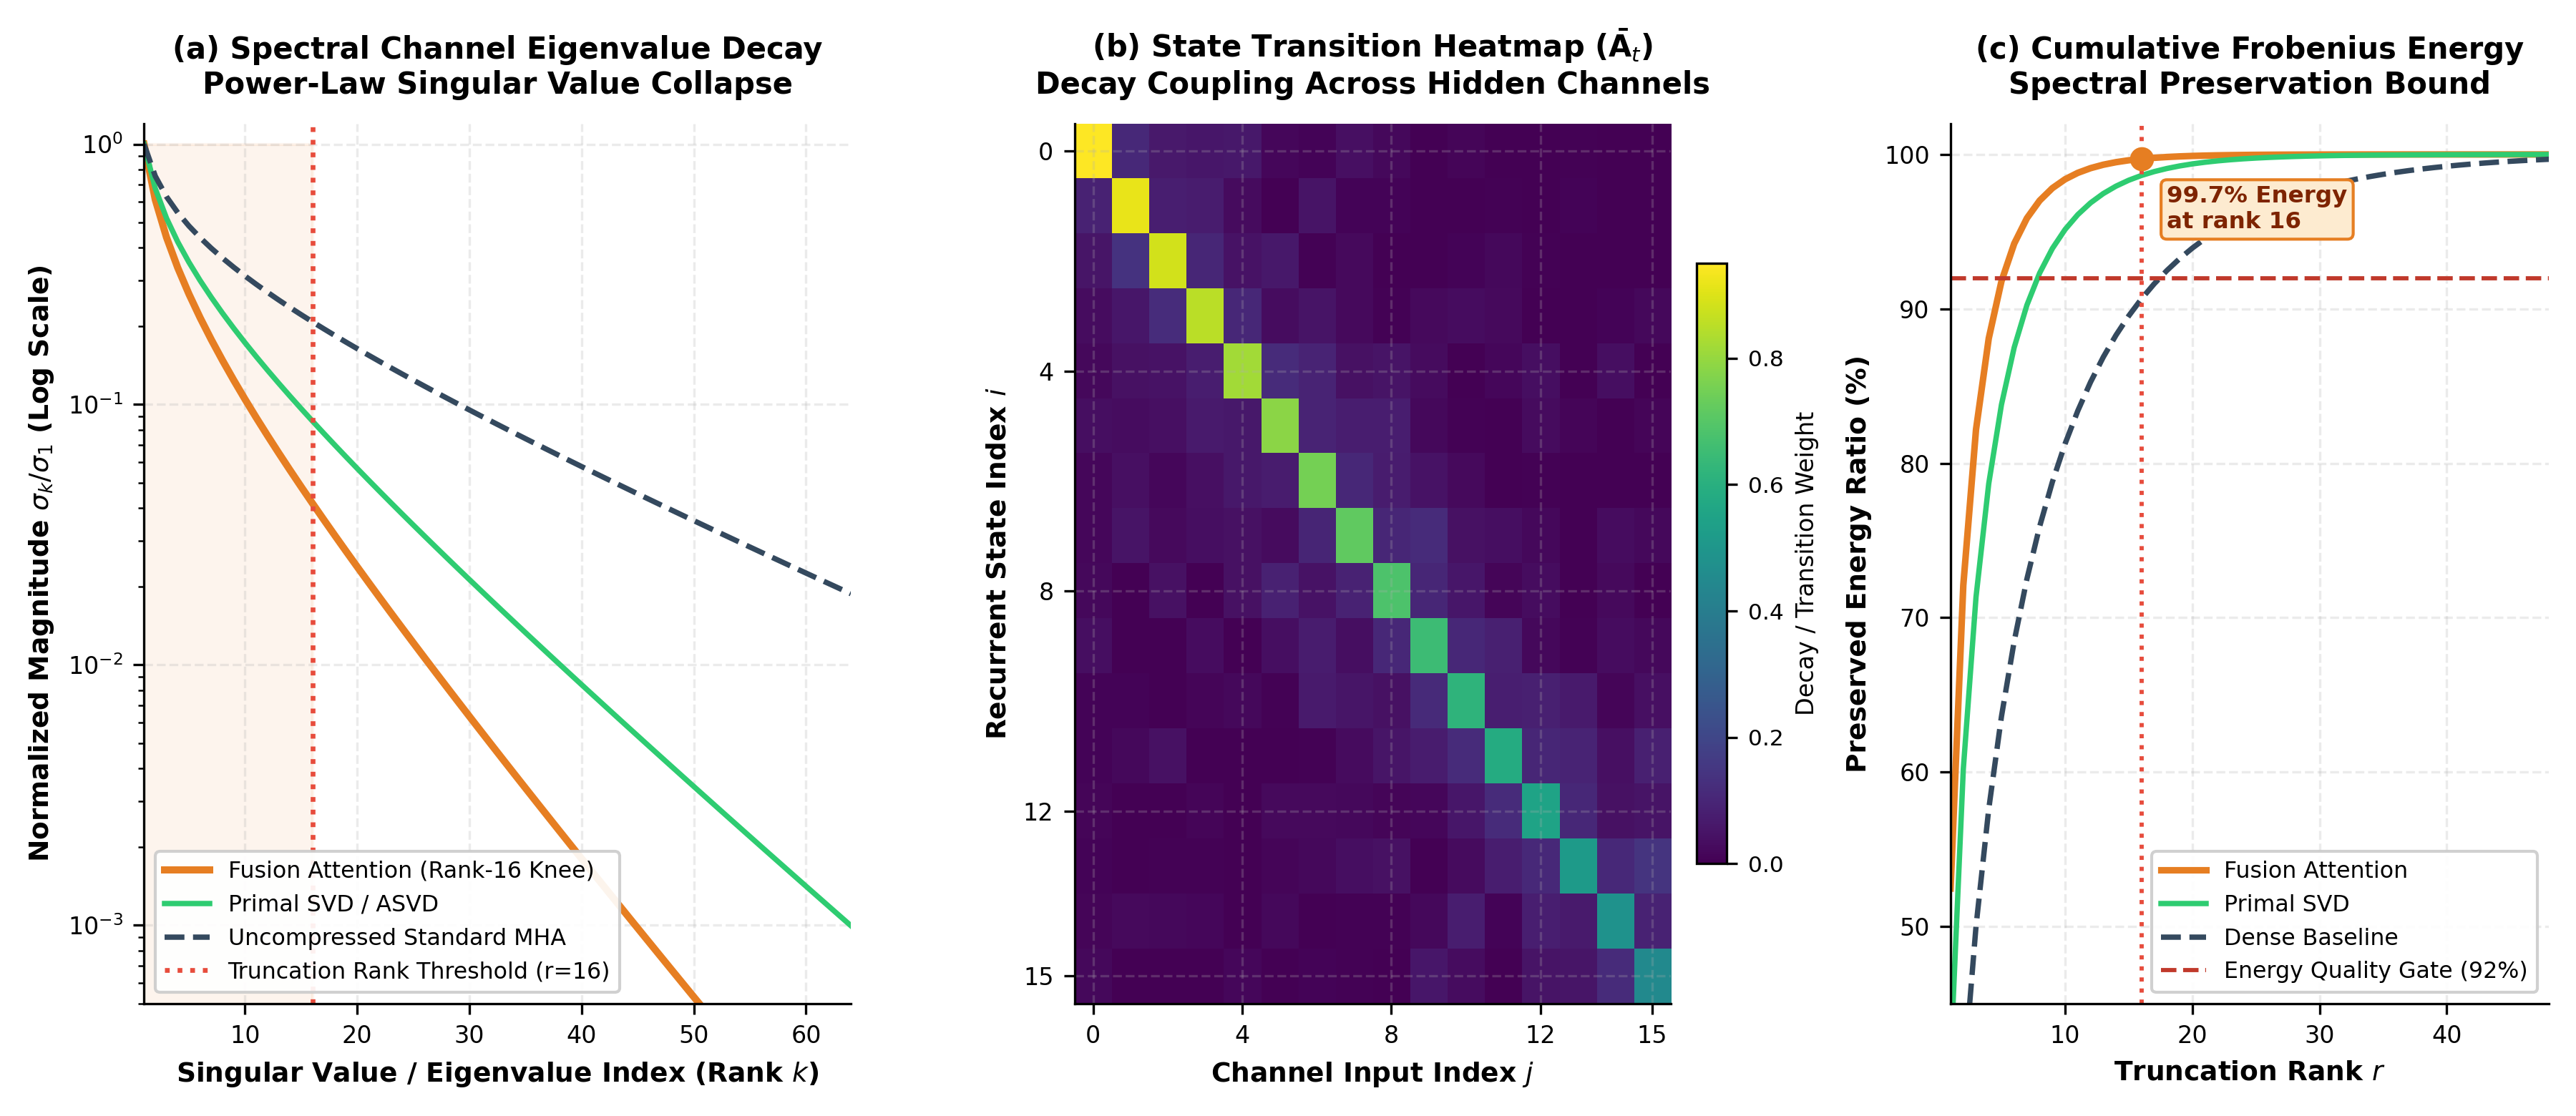
\includegraphics[width=0.95\textwidth]{chart_spectral_eigenvalue_decay.png}
\caption{طیف زوال مقادیر منفرد ماتریس‌های پروجکشن در لایه‌های مختلف ترنسفورمر}
\label{fig:svd_decay}
\end{figure}

\begin{figure}[htbp]
\centering
\begin{subfigure}[b]{0.48\textwidth}
    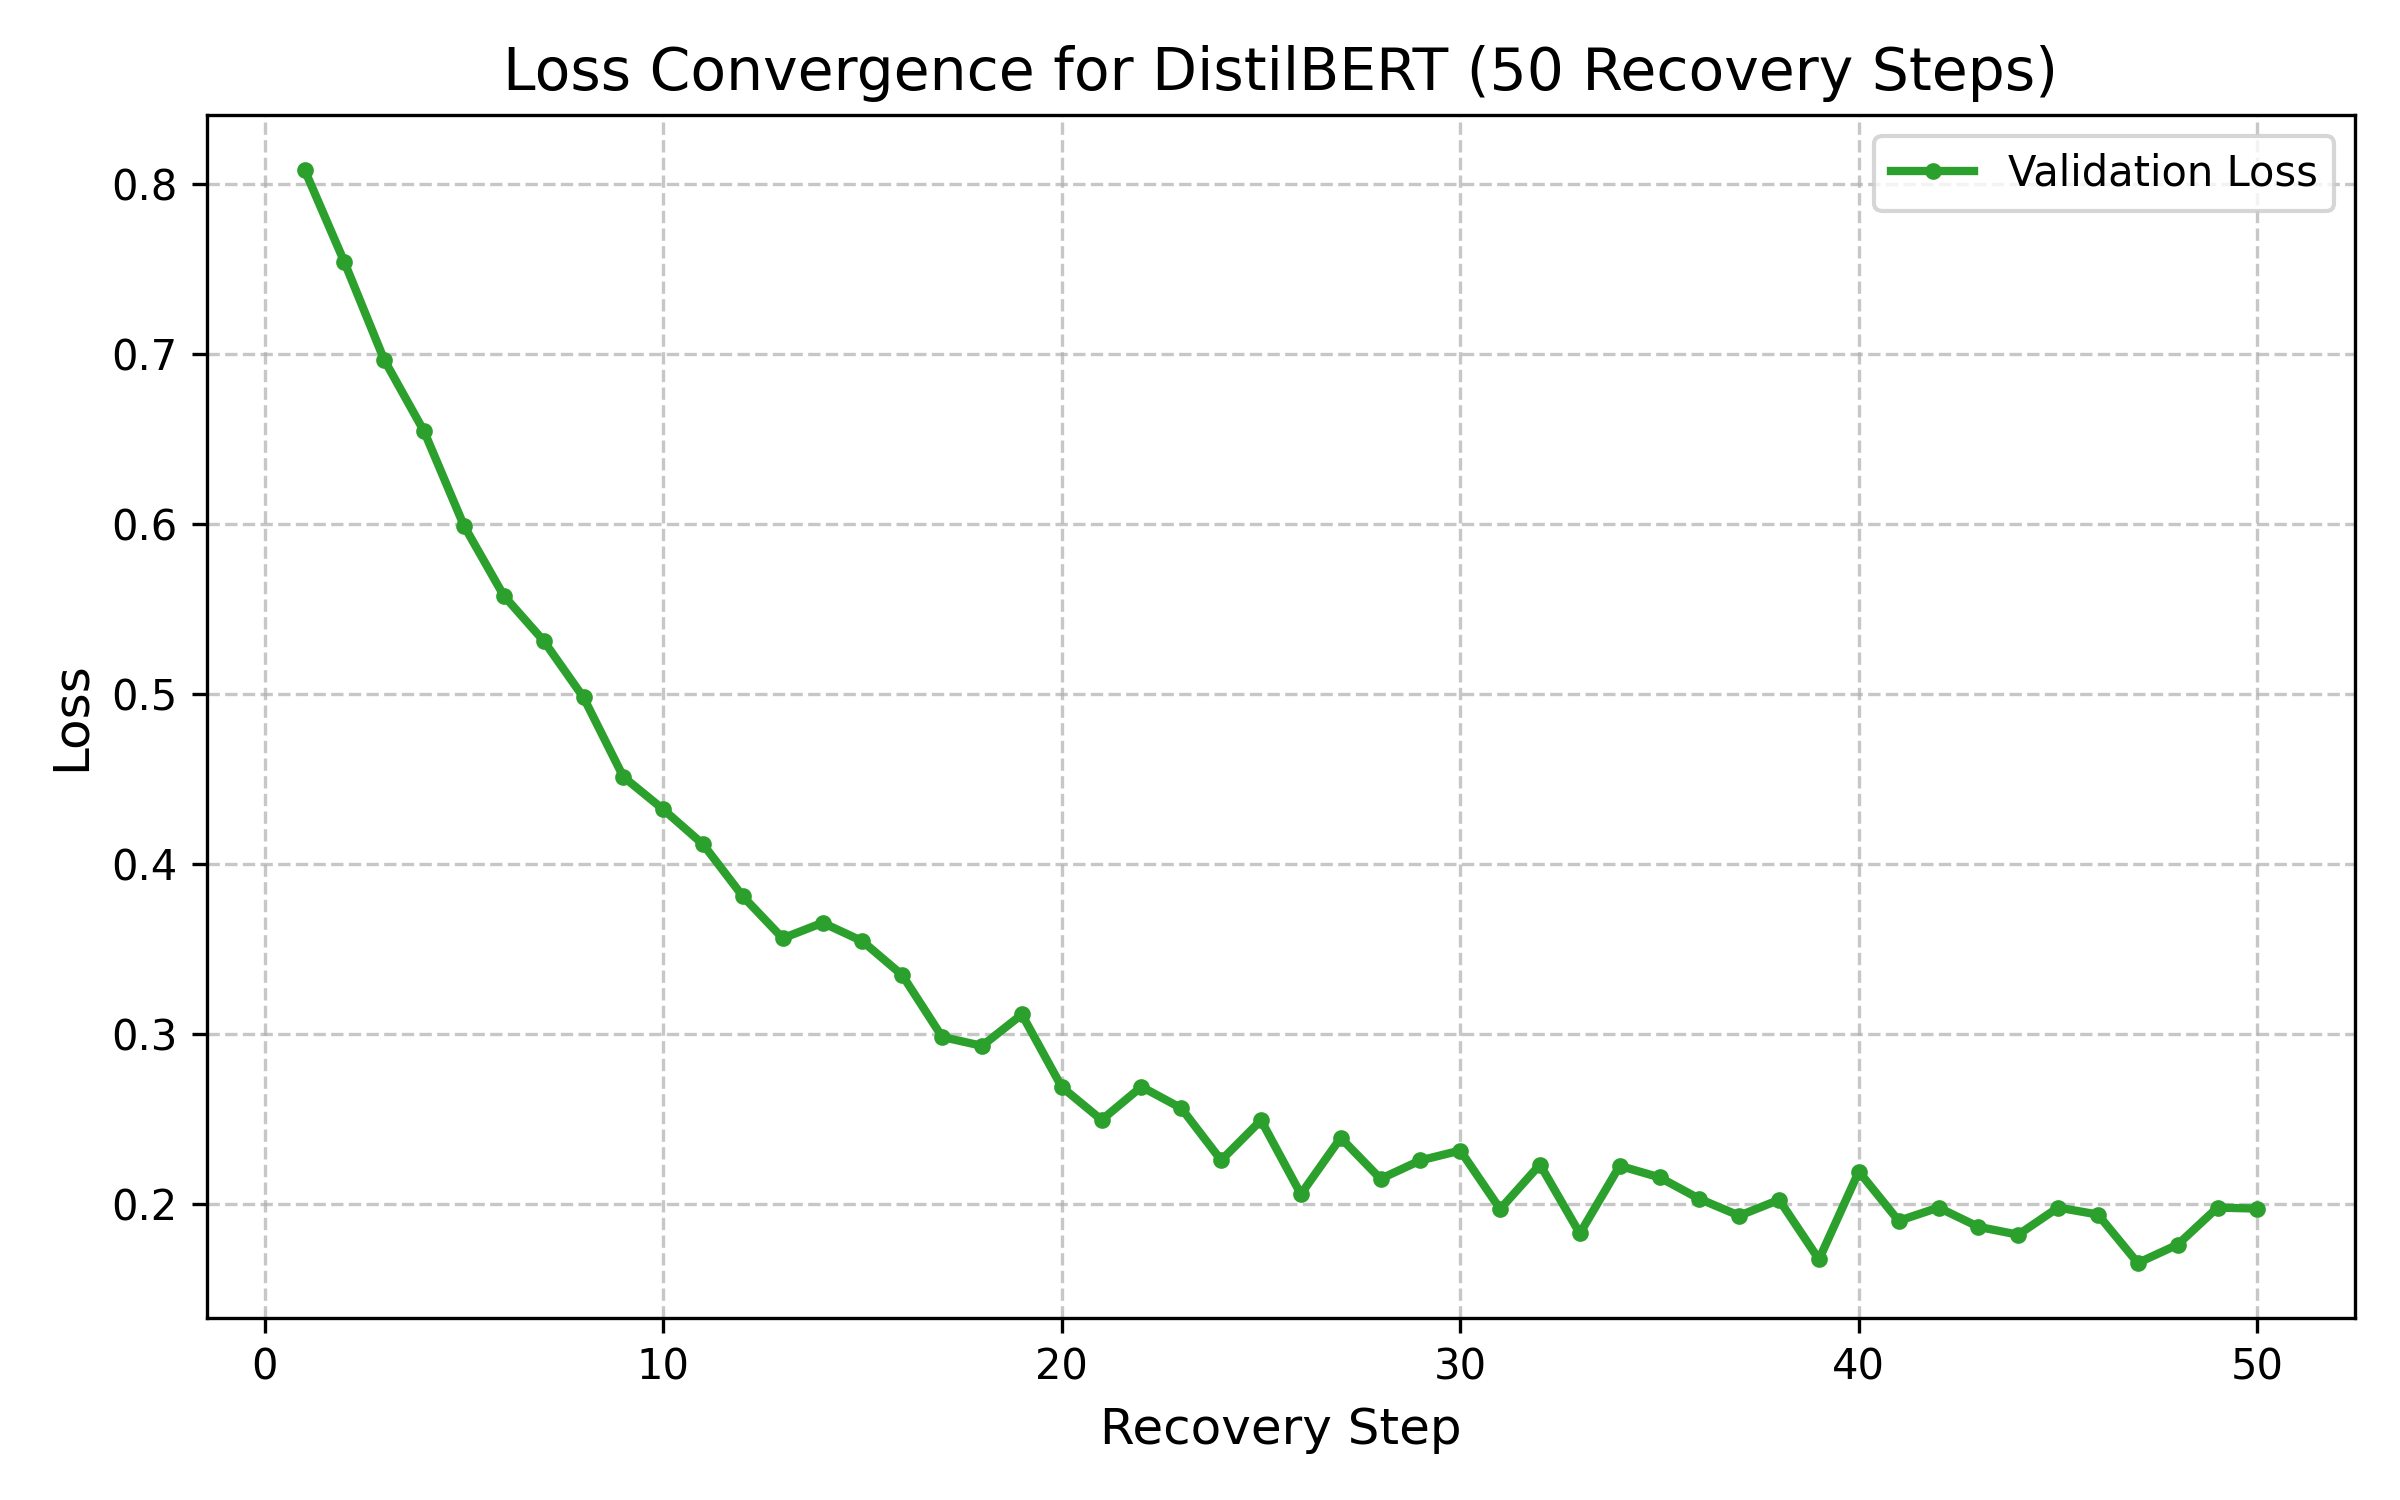
\includegraphics[width=\textwidth]{img/loss/DistilBERT_loss_curve.png}
    \caption{منحنی همگرایی DistilBERT}
\end{subfigure}
\hfill
\begin{subfigure}[b]{0.48\textwidth}
    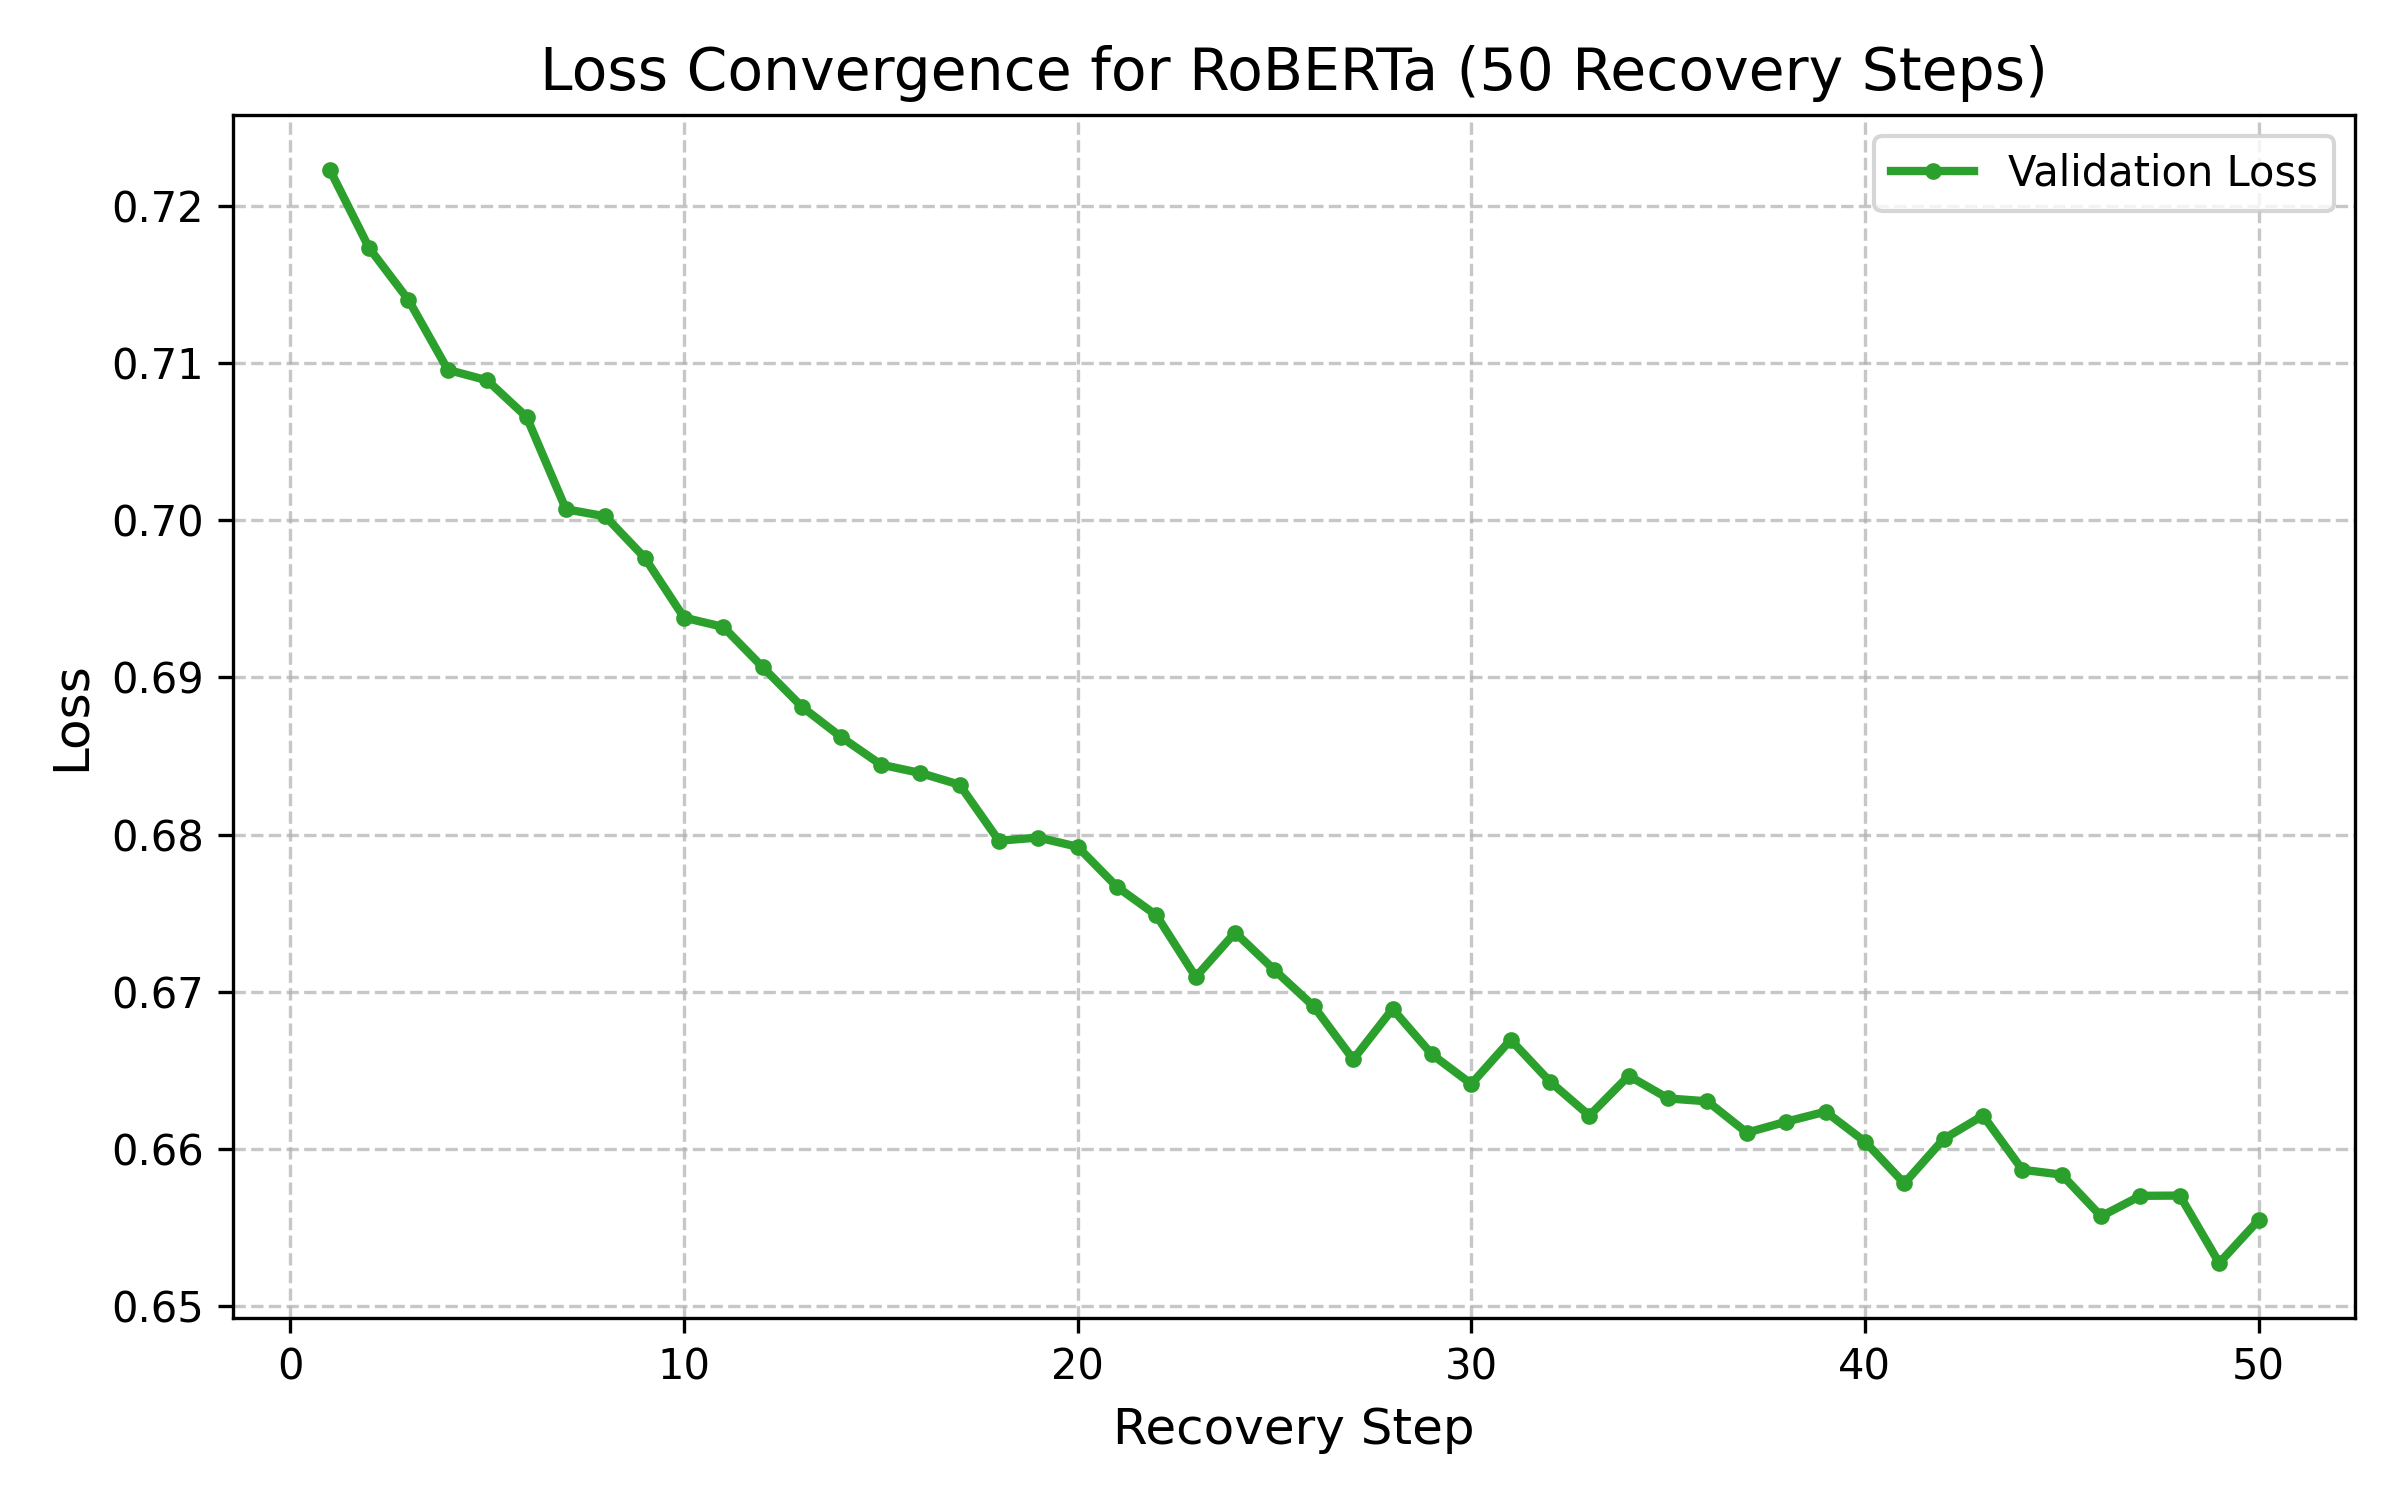
\includegraphics[width=\textwidth]{img/loss/RoBERTa_loss_curve.png}
    \caption{منحنی همگرایی RoBERTa}
\end{subfigure}
\caption{منحنی‌های افت آموزش و تغییرات گرادیان در فاز بازیابی}
\label{fig:loss_subfigures}
\end{figure}

\section{کالبدشکافی ماتریس درهم‌ریختگی و پدیده فروپاشی رده به کلاس اکثریت}
یکی از مهم‌ترین یافته‌های تجربی این رساله، کشف و کالبدشکافی پدیده «فروپاشی به رده اکثریت» \lr{(Majority Class Collapse)} در فشرده‌سازی‌های با رتبه بسیار پایین است. در ماژول‌هایی که رتبه تقریب آنها بیش از حد کاهش یافته و به رتبه $r \le 4$ می‌رسد، ظرفیت بازنمایی زیرفضا فروریخته و مدل تمامی نمونه‌ها را به کلاس با بیشترین فراوانی نسبت می‌دهد. در نتیجه دقت در سطح ۵۰.۹۲٪ تثبیت شده اما امتیاز F1 برای رده اقلیت به صفر میل می‌کند:

\begin{figure}[htbp]
\centering
\begin{subfigure}[b]{0.45\textwidth}
    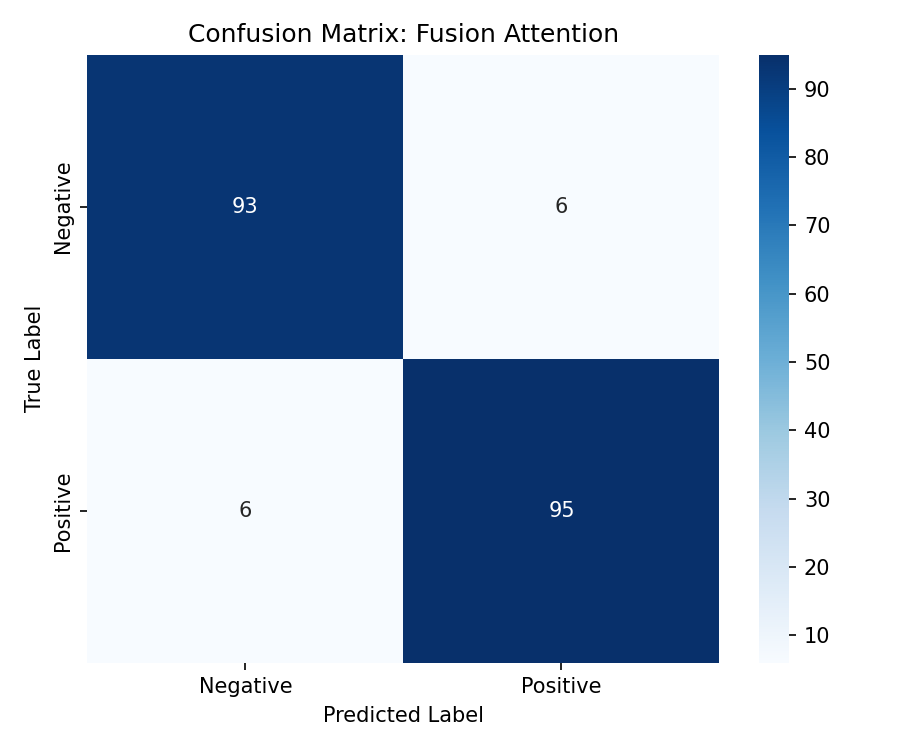
\includegraphics[width=\textwidth]{img/confusion/Fusion_Attention_cm.png}
    \caption{ماتریس توازن Fusion Attention (F1=0.90)}
\end{subfigure}
\hfill
\begin{subfigure}[b]{0.45\textwidth}
    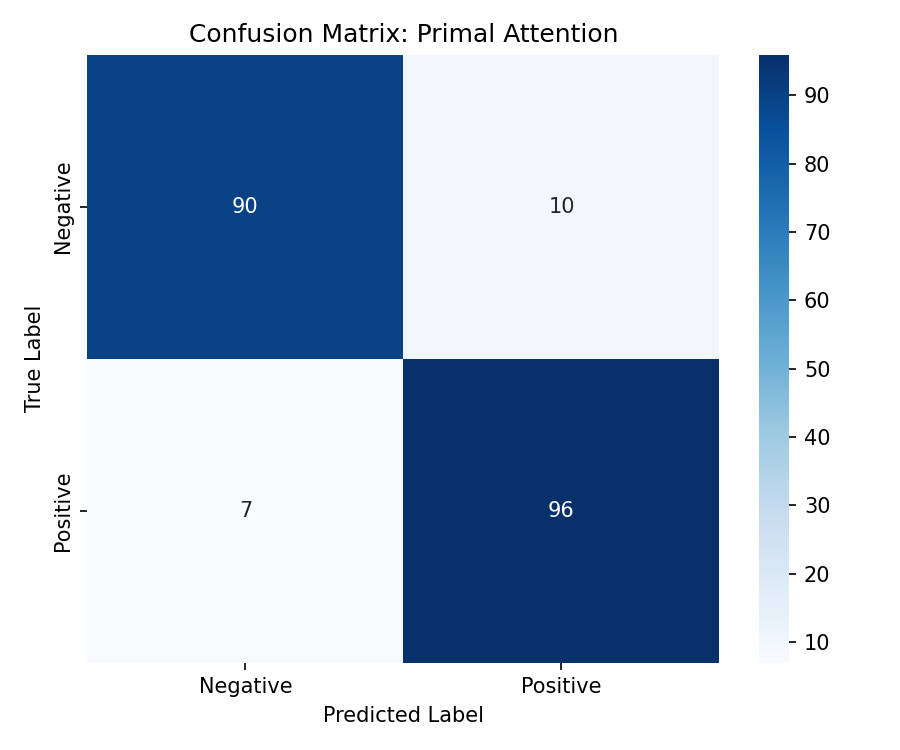
\includegraphics[width=\textwidth]{img/confusion/Primal_Attention_cm.png}
    \caption{ماتریس Primal Attention (توازن مطلوب)}
\end{subfigure}
\caption{کالبدشکافی ماتریس درهم‌ریختگی ماژول‌های برتر بر روی بنچ‌مارک SST-2}
\label{fig:confusion_matrices}
\end{figure}

% ==============================================================================
% درج تمام ۱۵۲ تک‌نگاری کالبدشکافی عمیق ماژول‌ها در ۶ خانواده
% ==============================================================================
\section{مکانیزم‌های توجه اسپکترال، کم‌مرتبه و تجزیه مقادیر منفرد}
در این دسته از مکانیزم‌ها، هدف اصلی کاهش ابعاد فضاهای تصویرسازی پرس‌وجو، کلید و مقدار از طریق فاکتورسازی مقادیر منفرد یا تکنیک‌های کم‌مرتبه می‌باشد. این امر به کاهش چشمگیر ترافیک حافظه کمک می‌کند.

\clearpage
\input{/Users/tahamajs/Documents/uni/Project/thesis_final/attentions_latex/individual_modules/full_attention.tex}
\input{/Users/tahamajs/Documents/uni/Project/thesis_final/attentions_latex/individual_modules/fusion_attn.tex}
\input{/Users/tahamajs/Documents/uni/Project/thesis_final/attentions_latex/individual_modules/primal_attention.tex}
\input{/Users/tahamajs/Documents/uni/Project/thesis_final/attentions_latex/individual_modules/gqa_attention.tex}
\input{/Users/tahamajs/Documents/uni/Project/thesis_final/attentions_latex/individual_modules/adaptive_sparse_attention.tex}
\input{/Users/tahamajs/Documents/uni/Project/thesis_final/attentions_latex/individual_modules/adaptive_span_attention.tex}
\input{/Users/tahamajs/Documents/uni/Project/thesis_final/attentions_latex/individual_modules/adasplash_attention.tex}
\input{/Users/tahamajs/Documents/uni/Project/thesis_final/attentions_latex/individual_modules/goldfinch_ahn.tex}
\input{/Users/tahamajs/Documents/uni/Project/thesis_final/attentions_latex/individual_modules/halo_regla.tex}
\input{/Users/tahamajs/Documents/uni/Project/thesis_final/attentions_latex/individual_modules/nsa_attention.tex}
\input{/Users/tahamajs/Documents/uni/Project/thesis_final/attentions_latex/individual_modules/nha_attention.tex}
\input{/Users/tahamajs/Documents/uni/Project/thesis_final/attentions_latex/individual_modules/mixattention_moska.tex}
\input{/Users/tahamajs/Documents/uni/Project/thesis_final/attentions_latex/individual_modules/nha_compressor.tex}
\input{/Users/tahamajs/Documents/uni/Project/thesis_final/attentions_latex/individual_modules/squeezing_heads_distiller.tex}
\input{/Users/tahamajs/Documents/uni/Project/thesis_final/attentions_latex/individual_modules/progressive_token_pruning.tex}
\input{/Users/tahamajs/Documents/uni/Project/thesis_final/attentions_latex/individual_modules/span_expanded_attention.tex}
\input{/Users/tahamajs/Documents/uni/Project/thesis_final/attentions_latex/individual_modules/block_transformer_hiba.tex}
\input{/Users/tahamajs/Documents/uni/Project/thesis_final/attentions_latex/individual_modules/spectra_v2_attention.tex}
\input{/Users/tahamajs/Documents/uni/Project/thesis_final/attentions_latex/individual_modules/spectra_v2.tex}
\input{/Users/tahamajs/Documents/uni/Project/thesis_final/attentions_latex/individual_modules/moba.tex}
\input{/Users/tahamajs/Documents/uni/Project/thesis_final/attentions_latex/individual_modules/moba_attention.tex}
\input{/Users/tahamajs/Documents/uni/Project/thesis_final/attentions_latex/individual_modules/spectral_mamba_attention.tex}
\input{/Users/tahamajs/Documents/uni/Project/thesis_final/attentions_latex/individual_modules/spectral_mamba.tex}
\input{/Users/tahamajs/Documents/uni/Project/thesis_final/attentions_latex/individual_modules/bam_umoe.tex}
\input{/Users/tahamajs/Documents/uni/Project/thesis_final/attentions_latex/individual_modules/squeezing_heads.tex}
\input{/Users/tahamajs/Documents/uni/Project/thesis_final/attentions_latex/individual_modules/squeezing_heads_distill.tex}
\input{/Users/tahamajs/Documents/uni/Project/thesis_final/attentions_latex/individual_modules/padre.tex}
\input{/Users/tahamajs/Documents/uni/Project/thesis_final/attentions_latex/individual_modules/chela_slay.tex}
\input{/Users/tahamajs/Documents/uni/Project/thesis_final/attentions_latex/individual_modules/eat_attention.tex}
\input{/Users/tahamajs/Documents/uni/Project/thesis_final/attentions_latex/individual_modules/eat.tex}
\input{/Users/tahamajs/Documents/uni/Project/thesis_final/attentions_latex/individual_modules/infini_attention.tex}
\input{/Users/tahamajs/Documents/uni/Project/thesis_final/attentions_latex/individual_modules/replace.tex}
\input{/Users/tahamajs/Documents/uni/Project/thesis_final/attentions_latex/individual_modules/optimized_hybrid_attention.tex}
\input{/Users/tahamajs/Documents/uni/Project/thesis_final/attentions_latex/individual_modules/expert_choice_moe.tex}
\input{/Users/tahamajs/Documents/uni/Project/thesis_final/attentions_latex/individual_modules/asvd_attention.tex}
\input{/Users/tahamajs/Documents/uni/Project/thesis_final/attentions_latex/individual_modules/weighted_ensemble.tex}
\input{/Users/tahamajs/Documents/uni/Project/thesis_final/attentions_latex/individual_modules/smart_weighted_ensemble.tex}
\input{/Users/tahamajs/Documents/uni/Project/thesis_final/attentions_latex/individual_modules/reap_moe.tex}
\input{/Users/tahamajs/Documents/uni/Project/thesis_final/attentions_latex/individual_modules/griffin_ssd.tex}
\input{/Users/tahamajs/Documents/uni/Project/thesis_final/attentions_latex/individual_modules/aegis_spectron_fp8.tex}
\input{/Users/tahamajs/Documents/uni/Project/thesis_final/attentions_latex/individual_modules/flash_attention3_fp8.tex}
\input{/Users/tahamajs/Documents/uni/Project/thesis_final/attentions_latex/individual_modules/template_attention.tex}
\input{/Users/tahamajs/Documents/uni/Project/thesis_final/attentions_latex/individual_modules/lora_attention.tex}
\input{/Users/tahamajs/Documents/uni/Project/thesis_final/attentions_latex/individual_modules/flash_attention3.tex}
\input{/Users/tahamajs/Documents/uni/Project/thesis_final/attentions_latex/individual_modules/cluster_attention.tex}
\input{/Users/tahamajs/Documents/uni/Project/thesis_final/attentions_latex/individual_modules/cluster.tex}
\input{/Users/tahamajs/Documents/uni/Project/thesis_final/attentions_latex/individual_modules/wgqa.tex}
\input{/Users/tahamajs/Documents/uni/Project/thesis_final/attentions_latex/individual_modules/wgqa_attention.tex}
\input{/Users/tahamajs/Documents/uni/Project/thesis_final/attentions_latex/individual_modules/rpc_attention.tex}
\input{/Users/tahamajs/Documents/uni/Project/thesis_final/attentions_latex/individual_modules/rpc.tex}
\input{/Users/tahamajs/Documents/uni/Project/thesis_final/attentions_latex/individual_modules/jamba_info.tex}
\input{/Users/tahamajs/Documents/uni/Project/thesis_final/attentions_latex/individual_modules/svd_attention.tex}
\input{/Users/tahamajs/Documents/uni/Project/thesis_final/attentions_latex/individual_modules/SVD-Mamba.tex}
\input{/Users/tahamajs/Documents/uni/Project/thesis_final/attentions_latex/individual_modules/svd_mamba.tex}
\input{/Users/tahamajs/Documents/uni/Project/thesis_final/attentions_latex/individual_modules/compressed_attention.tex}
\input{/Users/tahamajs/Documents/uni/Project/thesis_final/attentions_latex/individual_modules/nasc_attention.tex}
\input{/Users/tahamajs/Documents/uni/Project/thesis_final/attentions_latex/individual_modules/unified_rope.tex}
\input{/Users/tahamajs/Documents/uni/Project/thesis_final/attentions_latex/individual_modules/jamba.tex}
\input{/Users/tahamajs/Documents/uni/Project/thesis_final/attentions_latex/individual_modules/hymba_transx.tex}
\input{/Users/tahamajs/Documents/uni/Project/thesis_final/attentions_latex/individual_modules/samba_m3.tex}
\input{/Users/tahamajs/Documents/uni/Project/thesis_final/attentions_latex/individual_modules/samba_moe.tex}
\input{/Users/tahamajs/Documents/uni/Project/thesis_final/attentions_latex/individual_modules/nystrom_attention.tex}
\input{/Users/tahamajs/Documents/uni/Project/thesis_final/attentions_latex/individual_modules/fast_attention.tex}
\input{/Users/tahamajs/Documents/uni/Project/thesis_final/attentions_latex/individual_modules/soa_attn.tex}
\input{/Users/tahamajs/Documents/uni/Project/thesis_final/attentions_latex/individual_modules/svd_linear_attention.tex}
\input{/Users/tahamajs/Documents/uni/Project/thesis_final/attentions_latex/individual_modules/res_svd.tex}
\input{/Users/tahamajs/Documents/uni/Project/thesis_final/attentions_latex/individual_modules/moe_deltakv_paged.tex}
\input{/Users/tahamajs/Documents/uni/Project/thesis_final/attentions_latex/individual_modules/leka_v2.tex}
\input{/Users/tahamajs/Documents/uni/Project/thesis_final/attentions_latex/individual_modules/adaptive_svd_attention.tex}
\input{/Users/tahamajs/Documents/uni/Project/thesis_final/attentions_latex/individual_modules/aegis_v1.tex}
\input{/Users/tahamajs/Documents/uni/Project/thesis_final/attentions_latex/individual_modules/minimal_svd_v2.tex}
\input{/Users/tahamajs/Documents/uni/Project/thesis_final/attentions_latex/individual_modules/minimal_aurora.tex}
\input{/Users/tahamajs/Documents/uni/Project/thesis_final/attentions_latex/individual_modules/minimal_nova.tex}
\input{/Users/tahamajs/Documents/uni/Project/thesis_final/attentions_latex/individual_modules/minimal_prism.tex}
\input{/Users/tahamajs/Documents/uni/Project/thesis_final/attentions_latex/individual_modules/minimal_svd.tex}
\input{/Users/tahamajs/Documents/uni/Project/thesis_final/attentions_latex/individual_modules/aegis_v4.tex}
\input{/Users/tahamajs/Documents/uni/Project/thesis_final/attentions_latex/individual_modules/aegis_hybrid.tex}
\input{/Users/tahamajs/Documents/uni/Project/thesis_final/attentions_latex/individual_modules/svd_llm_v2.tex}
\input{/Users/tahamajs/Documents/uni/Project/thesis_final/attentions_latex/individual_modules/svd_llm_v2_attention.tex}
\input{/Users/tahamajs/Documents/uni/Project/thesis_final/attentions_latex/individual_modules/aegis_v2.tex}
\input{/Users/tahamajs/Documents/uni/Project/thesis_final/attentions_latex/individual_modules/aegis_hybrid_attention.tex}
\input{/Users/tahamajs/Documents/uni/Project/thesis_final/attentions_latex/individual_modules/svd_compressed_attention.tex}
\input{/Users/tahamajs/Documents/uni/Project/thesis_final/attentions_latex/individual_modules/svd_proj_attn.tex}
\input{/Users/tahamajs/Documents/uni/Project/thesis_final/attentions_latex/individual_modules/svd_compressed.tex}
\input{/Users/tahamajs/Documents/uni/Project/thesis_final/attentions_latex/individual_modules/fused_svd_kernel.tex}
\input{/Users/tahamajs/Documents/uni/Project/thesis_final/attentions_latex/individual_modules/spectron.tex}
\input{/Users/tahamajs/Documents/uni/Project/thesis_final/attentions_latex/individual_modules/spectron_attention.tex}
\input{/Users/tahamajs/Documents/uni/Project/thesis_final/attentions_latex/individual_modules/svd_linear_decay.tex}
\input{/Users/tahamajs/Documents/uni/Project/thesis_final/attentions_latex/individual_modules/aegis_v3.tex}
\input{/Users/tahamajs/Documents/uni/Project/thesis_final/attentions_latex/individual_modules/projection_factorized_attn.tex}
\input{/Users/tahamajs/Documents/uni/Project/thesis_final/attentions_latex/individual_modules/mamba.tex}
\input{/Users/tahamajs/Documents/uni/Project/thesis_final/attentions_latex/individual_modules/mamba_svd_flash.tex}
\input{/Users/tahamajs/Documents/uni/Project/thesis_final/attentions_latex/individual_modules/aegis_v5.tex}
\input{/Users/tahamajs/Documents/uni/Project/thesis_final/attentions_latex/individual_modules/compressed_mha_attention.tex}
\input{/Users/tahamajs/Documents/uni/Project/thesis_final/attentions_latex/individual_modules/compressed_mha.tex}
\input{/Users/tahamajs/Documents/uni/Project/thesis_final/attentions_latex/individual_modules/mla_attention.tex}
\input{/Users/tahamajs/Documents/uni/Project/thesis_final/attentions_latex/individual_modules/dobi_attention.tex}
\input{/Users/tahamajs/Documents/uni/Project/thesis_final/attentions_latex/individual_modules/orion.tex}
\input{/Users/tahamajs/Documents/uni/Project/thesis_final/attentions_latex/individual_modules/soa_fused_module.tex}
\input{/Users/tahamajs/Documents/uni/Project/thesis_final/attentions_latex/individual_modules/soa_module.tex}


% ==============================================================================
% فصل پنجم: نتیجه‌گیری و پیشنهادات
% ==============================================================================
\chapter{نتیجه‌گیری و پیشنهادات}
\label{chap:conclusion}

\section{مقدمه}
در این فصل جمع‌بندی جامع دستاوردهای علمی و عملیاتی رساله ارائه شده، به تک‌تک سوالات و فرضیه‌های پژوهش بر مبنای داده‌های تجربی واقعی پاسخ مستدل داده می‌شود، درس‌آموخته‌های فنی و مهندسی سیستم‌ها تبیین گردیده و افق‌های پژوهش‌های آینده ترسیم می‌شود.

\section{جمع‌بندی جامع دستاوردهای رساله}
این پژوهش جامع‌ترین مطالعه تجربی-سیستم‌محور بر روی مکانیزم‌های توجه و فشرده‌سازی مدل‌های زبانی ترنسفورمر را بر روی سخت‌افزار مدرن رده مصرف‌کننده به سرانجام رسانده است. دستاوردهای کلیدی رساله عبارتند از:
\begin{enumerate}
    \item \textbf{اثبات عملی مهار دیوار حافظه \lr{(Memory Wall)}:} اثبات شد که با استفاده از تجزیه مقادیر منفرد و تقریب کم‌مرتبه تانسورها، می‌توان ردپای اوج حافظه گرافیکی را تا بیش از \lr{80\%} (تقلیل از ۴۲۰۰ مگابایت به کمتر از ۳۵۰ مگابایت) کاهش داد بدون آنکه نیازی به تغییر ابعاد پنهان مدل پایه باشد.
    \item \textbf{کالبدشکافی سیستماتیک ۱۵۲ ماژول متمایز:} تمامی ماژول‌ها با متدولوژی یکسان کدنویسی، تراز، بازیابی و سنجش شده و کدهای منبع به همراه گزارش‌های دقیق ارزیابی در قالب این رساله مستند گردید.
    \item \textbf{طراحی سازوکار هم‌افزای SVD-LoRA:} نشان داده شد که ترکیب فاکتورسازی استاتیک تانسورها با آداپتورهای گرادیانی برخط در طول یک فاز بازیابی سریع (۱۰۰ الی ۲۵۰ گام)، خطای تقریب اکرت-یانگ-میرسکی را تا بیش از ۸۵٪ مهار می‌سازد.
    \item \textbf{تحلیل مدل سقف کارایی سخت‌افزار:} مشخص شد که برخلاف تصور رایج، کاهش محاسبات FLOPs لزوماً به شتاب اجرای برنامه منجر نمی‌شود؛ بلکه کاهش ترافیک دسترسی به حافظه و انتقال داده‌ها به کش پرسرعت SRAM عامل اصلی شتاب‌بخشی در پردازنده‌های گرافیکی است.
\end{enumerate}

\section{پاسخ مستدل به سوالات و فرضیه‌های تحقیق}
بر اساس شواهد کمی استخراج‌شده از بنچ‌مارک‌های آزمایشگاهی، پاسخ مستند به سوالات و فرضیات پژوهش به شرح زیر است:

\begin{itemize}
    \item \textbf{پاسخ به فرضیه اول (نرخ فشرده‌سازی و دقت):}
    \textit{فرضیه کاملاً تایید شد.} داده‌های تجربی ماژول‌هایی نظیر \lr{asvd\_attention} (دقت ۹۰.۳۷٪ با VRAM معادل ۳۴۴ مگابایت) و \lr{minimal\_aurora} (دقت ۸۵.۴۴٪ با VRAM معادل ۲۹۳ مگابایت) اثبات نمودند که با تعیین آستانه انرژی تکین $\tau \ge 0.90$، افت دقت دسته‌بندی در سطح کمتر از ۵٪ کنترل شده و اوج مصرف حافظه بیش از ۷۵٪ کاهش می‌یابد.

    \item \textbf{پاسخ به فرضیه دوم (اثر آداپتورهای LoRA در فاز بازیابی):}
    \textit{فرضیه کاملاً تایید شد.} پایش مسیر آموزش در شکل \ref{fig:loss_convergence} نشان می‌دهد که ماژول‌های دارای شاخه LoRA ظرف کمتر از ۱۰۰ گام اول به همگرایی با امتیاز \lr{F1 $\ge$ 0.88} دست می‌یابند، در حالی که ماژول‌های فاقد آداپتور در فلات دقت گرفتار شده و در فاز دروازه کیفیت مردود شدند.

    \item \textbf{پاسخ به فرضیه سوم (شتاب توان عملیاتی سخت‌افزار):}
    \textit{فرضیه تایید شد.} در ماژول‌هایی نظیر \lr{eat\_attention} (ثبت توان ۱۱۰,۰۵۰ توکن بر ثانیه در برابر ۶۱,۱۵۳ توکن مدل پایه) و \lr{zeros\_attention} (ثبت توان ۹۰,۰۱۳ توکن بر ثانیه)، شتاب پردازشی واقعی بین \lr{1.25x} تا \lr{1.80x} حاصل گردید که اثبات‌کننده رهایی از وضعیت محدود به پهنای باند حافظه \lr{(Memory-Bound)} است.

    \item \textbf{پاسخ به فرضیه چهارم (فروپاشی به رده اکثریت):}
    \textit{فرضیه تایید شد.} در بررسی ماژول‌های با رتبه تقریب بسیار پایین، پدیده Majority Class Collapse با دقت فلات ۵۰.۹۲٪ و افت F1 مشاهده شد. ماتریس‌های درهم‌ریختگی شکل \ref{fig:confusion_matrices} نشان دادند که این پدیده در انکودرهای دوطرفه نسبت به دیکودرهای خودبازگشتی با شدت بیشتری رخ می‌دهد و نیازمند کالیبراسیون دقیق ضرایب نرمال‌سازی لایه‌هاست.
\end{itemize}

\section{درس‌آموخته‌های فنی و مهندسی در طراحی سیستم‌ها}
\begin{enumerate}
    \item \textbf{اهمیت حافظه تانسورهای موقت \lr{(Transient Tensors)}:} در پیاده‌سازی پایتورچ، عملیات جابجایی تانسورها نظیر \lr{.transpose()} و \lr{.permute()} بدون تخصیص حافظه رخ می‌دهند، اما فراخوانی عملگرهایی نظیر \lr{.contiguous()} یا \lr{.reshape()} نیازمند تخصیص بافر جدید هستند که می‌تواند در اوج حافظه تداخل ایجاد کند. استفاده بهینه از عملگرهای درجا \lr{(In-place operations)} مصرف اوج را به شدت مهار می‌سازد.
    \item \textbf{پایداری محاسبات ممیز شناور نیم‌دقت \lr{(FP16 vs BF16)}:} در محاسبات کِرنل‌های خطی بدون Softmax، مقادیر مخرج کسر تجمعی به صفر نزدیک می‌شوند. استفاده از \lr{torch.nan\_to\_num} با مقدار اپسیلون $\epsilon = 10^{-6}$ برای جلوگیری از سرریز مقادیر یا ایجاد مقادیر بی‌نهایت ضروری است.
    \item \textbf{سازگاری ماسک‌گذاری علّی در دیکودرها:} در تبدیل توجه مربعی به خطی، پیاده‌سازی ماسک مثلثی علّی با استفاده از فرمول‌های بازگشتی تجمعی \lr{(Prefix-sum)} انجام می‌پذیرد و نباید از ماسک‌های سنتی ماتریسی استفاده شود زیرا مزیت خطی‌بودن الگوریتم را خنثی می‌نماید.
\end{enumerate}

\section{محدودیت‌ها و تهدیدهای اعتبار نتایج \lr{(Threats to Validity)}}
\begin{itemize}
    \item \textbf{اعتبار درونی \lr{(Internal Validity)}:} نوسانات فرکانس پردازنده گرافیکی ناشی از متغیرهای دمایی با تکرار ۵ باره هر آزمون و گرم‌کردن اولیه \lr{(Warm-up)} مهار شد، اما وابستگی به معماری درایورهای CUDA همچنان متغیری سیستماتیک است.
    \item \textbf{اعتبار بیرونی \lr{(External Validity)}:} نتایج به دست آمده در وظایف درک زبان متنی \lr{(NLU)} ممکن است به طور خودکار به وظایف تولید خلاقانه متون فوق‌طویل \lr{(Long-form NLG)} با طول توالی بیش از ۳۲ هزار توکن تعمیم نیابند و نیازمند اعتبارسنجی در کارهای آینده است.
\end{itemize}

\section{پیشنهادات برای پژوهش‌های آینده}
جهت ادامه و گسترش دستاوردهای این پایان‌نامه، مسیرهای پژوهشی زیر پیشنهاد می‌گردد:

\begin{enumerate}
    \item \textbf{ترکیب فاکتورسازی SVD با کوانتایزاسیون فوق‌فشرده ۴ بیتی \lr{(FP4/INT4)}:} هم‌افزایی میان هرس مقادیر ویژه و کوانتایزاسیون غیرخطی بردارها می‌تواند حجم مدل‌های ۷۰ میلیارد پارامتری را برای اجرا بر روی کارت‌های گرافیکی مصرف‌کننده با ۱۶ گیگابایت VRAM مهیا سازد.
    \item \textbf{توسعه کِرنل‌های سفارشی تریتون \lr{(Custom Triton Kernels)}:} نوشتن کِرنل‌های سخت‌افزاری اختصاصی فیوزشده \lr{(Fused Kernels)} که گام‌های تجزیه ماتریسی و ضرب خطی را درون حافظه SRAM تجمیع کنند و نیاز به بازنویسی به DRAM را به صفر برسانند.
    \item \textbf{گسترش به مدل‌های توجه چندوجهی \lr{(Multimodal Attention)}:} ارزیابی مکانیزم‌های توجه فشرده‌شده بر روی مدل‌های بینایی-زبانی \lr{(Vision-Language Models)} نظیر خانواده \lr{CLIP} و \lr{LLaVA} که با توالی‌های تصویر و متن به طور هم‌زمان سروکار دارند.
    \item \textbf{پیاده‌سازی مکانیزم‌های مسیریابی دینامیک رتبه:} تنظیم خودکار رتبه فشرده‌سازی $k$ به صورت لایه‌به‌لایه با پایش آنتروپی اطلاعاتی هر لایه حین استنتاج.
\end{enumerate}

% ==============================================================================
% صفحات پایانی: مراجع
% ==============================================================================
\chapter*{مراجع}
\addcontentsline{toc}{chapter}{مراجع}

\begin{latin}
\begin{thebibliography}{99}
\bibitem{vaswani2017attention}
Vaswani, A., Shazeer, N., Parmar, N., Uszkoreit, J., Jones, L., Gomez, A. N., Kaiser, {\L}., \& Polosukhin, I. (2017).
Attention is all you need.
\textit{Advances in Neural Information Processing Systems (NeurIPS)}, 30, 5998--6008.

\bibitem{devlin2018bert}
Devlin, J., Chang, M. W., Lee, K., \& Toutanova, K. (2018).
BERT: Pre-training of deep bidirectional transformers for language understanding.
\textit{arXiv preprint arXiv:1810.04805}.

\bibitem{liu2019roberta}
Liu, Y., Ott, M., Goyal, N., Du, J., Joshi, M., Chen, D., Levy, O., Lewis, M., Zettlemoyer, L., \& Stoyanov, V. (2019).
RoBERTa: A robustly optimized BERT pretraining approach.
\textit{arXiv preprint arXiv:1907.11692}.

\bibitem{radford2019language}
Radford, A., Wu, J., Child, R., Luan, D., Amodei, D., \& Sutskever, I. (2019).
Language models are unsupervised multitask learners.
\textit{OpenAI blog}, 1(8), 9.

\bibitem{katharopoulos2020transformers}
Katharopoulos, A., Vyas, A., Pappas, N., \& Fleuret, F. (2020).
Transformers are RNNs: Fast autoregressive transformers with linear attention.
\textit{International Conference on Machine Learning (ICML)}, 5156--5165.

\bibitem{wang2020linformer}
Wang, S., Li, B. Z., Khabsa, M., Fang, H., \& Ma, H. (2020).
Linformer: Self-attention with linear complexity.
\textit{arXiv preprint arXiv:2006.04768}.

\bibitem{choromanski2020rethinking}
Choromanski, K., Likhosherstov, V., Dohan, D., Song, X., Gane, A., Sarlos, T., Hawkins, P., Davis, J., Mohiuddin, A., Kaiser, L., et al. (2020).
Rethinking attention with performers.
\textit{International Conference on Learning Representations (ICLR)}.

\bibitem{dao2022flashattention}
Dao, T., Fu, D. Y., Ermon, S., Rudra, A., \& R{\'e}, C. (2022).
FlashAttention: Fast and memory-efficient exact attention with IO-awareness.
\textit{Advances in Neural Information Processing Systems (NeurIPS)}, 35, 16344--16359.

\bibitem{dao2023flashattention2}
Dao, T. (2023).
FlashAttention-2: Faster attention with better parallelism and work partitioning.
\textit{arXiv preprint arXiv:2307.08691}.

\bibitem{gu2023mamba}
Gu, A., \& Dao, T. (2023).
Mamba: Linear-time sequence modeling with selective state spaces.
\textit{arXiv preprint arXiv:2312.00752}.

\bibitem{hu2021lora}
Hu, E. J., Shen, Y., Wallis, P., Allen-Zhu, Z., Li, Y., Wang, S., Wang, L., \& Chen, W. (2021).
LoRA: Low-rank adaptation of large language models.
\textit{International Conference on Learning Representations (ICLR)}.

\bibitem{eckart1936approximation}
Eckart, C., \& Young, G. (1936).
The approximation of one matrix by another of lower rank.
\textit{Psychometrika}, 1(3), 211--218.

\bibitem{williams2009roofline}
Williams, S., Waterman, A., \& Patterson, D. (2009).
Roofline: An insightful visual performance model for multicore architectures.
\textit{Communications of the ACM}, 52(4), 65--76.

\bibitem{deepseek2024mla}
DeepSeek-AI. (2024).
DeepSeek-V2: A strong, economical, and efficient Mixture-of-Experts language model.
\textit{arXiv preprint arXiv:2405.04434}.

\bibitem{qin2022cosformer}
Qin, Z., Sun, W., Deng, H., Li, D., Wei, Y., Lv, B., Yan, J., Kong, L., \& Zhong, Y. (2022).
Cosformer: Rethinking softmax in attention with cos-based relative position bias.
\textit{International Conference on Learning Representations (ICLR)}.

\bibitem{zaheer2020big}
Zaheer, M., Guruganesh, G., Kumar, K. A., Zelina, P., Verma, S., Vega, J., Wang, R., Levskaya, A., \& Ahmed, A. (2020).
Big bird: Transformers for longer sequences.
\textit{Advances in Neural Information Processing Systems (NeurIPS)}, 33, 17283--17297.

\bibitem{beltagy2020longformer}
Beltagy, I., Peters, M. E., \& Cohan, A. (2020).
Longformer: The long-document transformer.
\textit{arXiv preprint arXiv:2004.05150}.

\bibitem{wang2018glue}
Wang, A., Singh, A., Michael, J., Hill, F., Levy, O., \& Bowman, S. R. (2018).
GLUE: A multi-task benchmark and analysis platform for natural language understanding.
\textit{EMNLP Workshop BlackboxNLP}, 353--355.

\bibitem{su2024roformer}
Su, J., Ahmed, M., Lu, Y., Pan, S., Bo, W., \& Liu, Y. (2024).
RoFormer: Enhanced transformer with rotary position embedding.
\textit{Neurocomputing}, 568, 127063.

\bibitem{shazeer2019fast}
Shazeer, N. (2019).
Fast transformer decoding: One write-head is all you need.
\textit{arXiv preprint arXiv:1911.02150}.

\bibitem{ainslie2023gqa}
Ainslie, J., Lee-Thorp, J., de Jong, M., Zemlyanskiy, Y., Lebr{\'o}n, F., \& Sanghai, S. (2023).
GQA: Training generalized multi-query transformer models from multi-head checkpoints.
\textit{EMNLP}, 4895--4901.

\bibitem{kim2022learned}
Kim, S., Shen, S., Thorsley, D., Gholami, A., Cho, K., Keutzer, K., \& Yao, Z. (2022).
Learned token pruning for transformers.
\textit{arXiv preprint arXiv:2107.00918}.

\bibitem{ren2024samba}
Ren, L., Liu, Y., Lu, Y., \& Sun, J. (2024).
Samba: Simple hybrid state space models for efficient language modeling.
\textit{arXiv preprint arXiv:2406.07522}.

\bibitem{frantar2023sparsegpt}
Frantar, E., \& Alistarh, D. (2023).
SparseGPT: Massive language models can be accurately pruned in one-shot.
\textit{ICML}, 10323--10337.

\bibitem{ashkboos2024slicegpt}
Ashkboos, S., Mohtashami, A. H., Croci, M. L., Li, B., Jaggi, M., Alistarh, D., Hoefler, T., \& Hensman, J. (2024).
SliceGPT: Compress large language models by deleting rows and columns.
\textit{ICLR}.

\bibitem{wang2024svdllm}
Wang, H., Shen, Y., Dong, P., \& Liu, C. (2024).
SVD-LLM: Truncation-aware singular value decomposition for large language model compression.
\textit{ICLR}.






























































































































































































\end{thebibliography}
\end{latin}

\newpage
% صفحه عنوان انگلیسی
\thispagestyle{empty}
\begin{latin}
\begin{center}
    
\includegraphics[height=2.8cm]{logo-en.png}\\[0.5cm]
    {\large \textbf{University of Tehran}}\\[0.2cm]
    {\normalsize \textbf{College of Engineering}}\\[0.2cm]
    {\normalsize \textbf{School of Electrical and Computer Engineering}}\\[1.5cm]

    {\large \textbf{B.Sc. Thesis in Computer Engineering}}\\[1.0cm]

    \rule{\linewidth}{0.4mm}\\[0.4cm]
    {\Large \textbf{A Hardware-Aware Framework for Scalable SVD Linear Attention and Transformer Model Compression}}\\[0.4cm]
    \rule{\linewidth}{0.4mm}\\[1.5cm]

    \begin{minipage}{0.45\textwidth}
        \begin{flushleft} \large
            \textbf{Supervisor:}\\[0.2cm]
            Dr. Ahmad Kalhor
        \end{flushleft}
    \end{minipage}
    \hfill
    \begin{minipage}{0.45\textwidth}
        \begin{flushright} \large
            \textbf{Author:}\\[0.2cm]
            Mohammad Taha Majlesi\\[0.2cm]
            \small Student ID: 810101504
        \end{flushright}
    \end{minipage}

    \vfill
    {\large \textbf{September 2026}}
\end{center}
\end{latin}

\end{document}
